\documentclass[journal]{IEEEtran}
\usepackage[T1]{fontenc}
\usepackage[utf8]{inputenc}
\usepackage{cite,amsmath,amssymb,booktabs,array,tabularx,url,textcomp}
\usepackage{graphicx}
\newcolumntype{L}[1]{>{\raggedright\arraybackslash}p{#1}}
\newcolumntype{Y}{>{\raggedright\arraybackslash}X}
\newcommand{\surveytableformat}{%
  \footnotesize
  \setlength{\tabcolsep}{5pt}%
  \renewcommand{\arraystretch}{1.12}%
}
\newcommand{\surveytablepair}[2]{#1\par\textit{#2}}
\newcommand{\surveytableinputs}[2]{#1\par\textit{Inputs:} #2}
\newcommand{\surveyplatformnote}{%
  \par\vspace{3pt}%
  \parbox{\linewidth}{\footnotesize\raggedright
    Superscripts mark evaluations on road vehicles (R), other ground robots (G), and non-ground, handheld, mixed, or unspecified carriers (N).}%
}
\setlength{\textfloatsep}{12pt plus 2pt minus 2pt}
\setlength{\dbltextfloatsep}{12pt plus 2pt minus 2pt}
\setlength{\floatsep}{10pt plus 2pt minus 2pt}
\setlength{\dblfloatsep}{10pt plus 2pt minus 2pt}
\DeclareUnicodeCharacter{2010}{-}
\DeclareUnicodeCharacter{2011}{-}
\DeclareUnicodeCharacter{2013}{--}
\DeclareUnicodeCharacter{2014}{---}
\DeclareUnicodeCharacter{2212}{-}
\hyphenation{local-iza-tion re-local-iza-tion tra-vers-a-bil-ity multi-robot}

\usepackage{xr}
% Tables S3--S7 live in the supplement. Build supplement.tex before survey.tex.
\externaldocument[S-]{supplement}
% Generated by scripts/build_data.py; counts describe this sample.
\newcommand{\CorpusCount}{245}
\newcommand{\CoreCount}{244}
\newcommand{\ContextCount}{1}
\newcommand{\BackgroundCount}{25}
\newcommand{\BaselineCount}{45}
\newcommand{\SupplementCount}{5}
\newcommand{\ExpansionCount}{60}
\newcommand{\FollowupCount}{15}
\newcommand{\IEEECount}{20}
\newcommand{\SurveyExpansionCount}{48}
\newcommand{\IEEERefreshCount}{36}
\newcommand{\JournalCount}{201}
\newcommand{\ConferenceCount}{44}
\newcommand{\FullCount}{23}
\newcommand{\LightCount}{222}
\newcommand{\LegacyLightCount}{87}
\newcommand{\TargetedLightCount}{135}
\newcommand{\BoundaryCount}{73}
\newcommand{\TargetCount}{172}
\newcommand{\ClosedCount}{123}
\newcommand{\RecordedCount}{54}
\newcommand{\PlaybackCount}{23}
\newcommand{\OnlineCount}{12}
\newcommand{\SimulationCount}{12}
\newcommand{\NumericalCount}{11}
\newcommand{\ResourceCount}{9}
\newcommand{\SurveyCount}{1}
\newcommand{\LocalizationCount}{67}
\newcommand{\PlanningCount}{57}
\newcommand{\SemanticCount}{36}
\newcommand{\MultiCount}{45}
\newcommand{\ReliabilityCount}{40}
\newcommand{\LegacyRecords}{58,583}
\newcommand{\LegacyReviewable}{43,086}
\newcommand{\LegacyUnreviewed}{43,041}
\newcommand{\LegacyJournals}{17}
\newcommand{\LegacySlices}{102}
\newcommand{\HistoricalQueue}{79}
\newcommand{\QuerySlices}{34}
\newcommand{\QueryIncomplete}{7}
\newcommand{\OnboardCount}{44}
\newcommand{\CoverageCount}{16}
\newcommand{\RecentCount}{173}
\newcommand{\RecentShare}{71}
\newcommand{\LocTechCount}{67}
\newcommand{\LocTaskCount}{1}
\newcommand{\LocNamedCount}{61}
\newcommand{\LocSameCount}{1}
\newcommand{\LocSameShare}{1}
\newcommand{\LocPhysSameCount}{1}
\newcommand{\LocIntegrityCount}{3}
\newcommand{\LocNonWheeledCount}{37}
\newcommand{\PlnTechCount}{56}
\newcommand{\PlnTaskCount}{44}
\newcommand{\PlnNamedCount}{46}
\newcommand{\PlnSameCount}{36}
\newcommand{\PlnSameShare}{64}
\newcommand{\PlnPhysSameCount}{20}
\newcommand{\PlnIntegrityCount}{1}
\newcommand{\PlnNonWheeledCount}{6}
\newcommand{\SemTechCount}{36}
\newcommand{\SemTaskCount}{33}
\newcommand{\SemNamedCount}{19}
\newcommand{\SemSameCount}{17}
\newcommand{\SemSameShare}{47}
\newcommand{\SemPhysSameCount}{13}
\newcommand{\SemIntegrityCount}{0}
\newcommand{\SemNonWheeledCount}{6}
\newcommand{\MrcTechCount}{45}
\newcommand{\MrcTaskCount}{25}
\newcommand{\MrcNamedCount}{27}
\newcommand{\MrcSameCount}{11}
\newcommand{\MrcSameShare}{24}
\newcommand{\MrcPhysSameCount}{2}
\newcommand{\MrcIntegrityCount}{1}
\newcommand{\MrcNonWheeledCount}{13}
\newcommand{\RelTechCount}{40}
\newcommand{\RelTaskCount}{20}
\newcommand{\RelNamedCount}{34}
\newcommand{\RelSameCount}{16}
\newcommand{\RelSameShare}{40}
\newcommand{\RelPhysSameCount}{7}
\newcommand{\RelIntegrityCount}{9}
\newcommand{\RelNonWheeledCount}{10}
\newcommand{\DegTaskCount}{81}
\newcommand{\DegTaskShare}{33}
\newcommand{\TaskAnyCount}{123}
\newcommand{\NamedCount}{187}
\newcommand{\AddressedCount}{219}
\newcommand{\ManipulatedCount}{61}
\newcommand{\SelectedOnlyCount}{126}
\newcommand{\IncidentalOnlyCount}{10}
\newcommand{\DOneSameCount}{27}
\newcommand{\PhysSameCount}{43}
\newcommand{\DirectWheeledCount}{37}
\newcommand{\IntegrityCount}{14}
\newcommand{\ComputeUnreported}{89}
\newcommand{\GroupWHL}{172}
\newcommand{\GroupROAD}{12}
\newcommand{\GroupGND}{13}
\newcommand{\GroupOTH}{47}
\newcommand{\DrivetrainEffectCount}{10}
\newcommand{\DOneSameShare}{11}
\newcommand{\DTwoSameCount}{54}
\newcommand{\LocNamedShare}{91}
\newcommand{\DrivetrainRecheckAdded}{4}
\newcommand{\LevelRecheckWorks}{19}
\newcommand{\LevelRecheckRevised}{2}
\newcommand{\LocatorCorrectionWorks}{2}
\newcommand{\SettingRecheckRevised}{5}
\newcommand{\DOneNominalShare}{5}
\newcommand{\AnyUnitShare}{34}
\newcommand{\IncidentalShare}{36}
\newcommand{\DegTaskCountCard}{61}
\newcommand{\DegTaskShareCard}{25}
\newcommand{\DepthFullShare}{30}
\newcommand{\DepthLegacyShare}{38}
\newcommand{\DepthTargetedShare}{30}
\newcommand{\WhlShare}{40}
\newcommand{\NonWhlShare}{17}
\newcommand{\QuotaShare}{34}
\newcommand{\NonQuotaShare}{32}
\newcommand{\NoIEEEOnlyShare}{33}
\newcommand{\StageMinShare}{32}
\newcommand{\StageMaxShare}{35}
\newcommand{\YearMinShare}{23}
\newcommand{\YearMaxShare}{46}
\newcommand{\DegTaskCountBase}{77}
\newcommand{\CoreCountBase}{228}
\newcommand{\DegTaskShareBase}{34}
\newcommand{\IfaceOneRank}{4}
\newcommand{\IfaceOneRankA}{4}
\newcommand{\IfaceOneRankB}{5}
\newcommand{\IfaceOneWorks}{15}
\newcommand{\IfaceOneDirect}{1}
\newcommand{\IfaceTwoRank}{10}
\newcommand{\IfaceTwoRankA}{8}
\newcommand{\IfaceTwoRankB}{26}
\newcommand{\IfaceTwoWorks}{11}
\newcommand{\IfaceTwoDirect}{6}
\newcommand{\IfaceThreeRank}{11}
\newcommand{\IfaceThreeRankA}{9}
\newcommand{\IfaceThreeRankB}{18}
\newcommand{\IfaceThreeWorks}{6}
\newcommand{\IfaceThreeDirect}{1}
\newcommand{\IfaceFourRank}{1}
\newcommand{\IfaceFourRankA}{1}
\newcommand{\IfaceFourRankB}{12}
\newcommand{\IfaceFourWorks}{17}
\newcommand{\IfaceFourDirect}{0}
\newcommand{\CandidateCount}{32}
\newcommand{\RejectedCount}{6}
\newcommand{\IfaceBestRank}{1}
\newcommand{\IfaceWorstRank}{11}
\newcommand{\HumanAssistCount}{10}
\newcommand{\IfaceTwoResRank}{26}
\newcommand{\IfaceThreeTerWorks}{2}
\newcommand{\IfaceFourWhl}{12}
\newcommand{\DegTaskCountPrimary}{81}
\newcommand{\IEEEShare}{72}
\newcommand{\IEEEOnlyCount}{56}
\newcommand{\IEEEShareRest}{64}
\newcommand{\BaselineIEEE}{38}
\newcommand{\SupplementIEEE}{3}
\newcommand{\ExpansionIEEE}{42}
\newcommand{\FollowupIEEE}{8}
\newcommand{\TargetedIEEE}{20}
\newcommand{\SurveyExpansionIEEE}{21}
\newcommand{\RefreshIEEE}{36}
\newcommand{\CoverageIEEE}{9}
\newcommand{\TotalIEEE}{177}
\newcommand{\SampleCount}{40}
\newcommand{\KappaMedian}{0.81}
\newcommand{\KappaMin}{$-$0.04}
\newcommand{\KappaMax}{1.00}
\newcommand{\AgreeMin}{67.5}
\newcommand{\AgreeMax}{100.0}
\newcommand{\DisagreeCount}{112}
\newcommand{\ResolvedPrimary}{58}
\newcommand{\ResolvedSecond}{46}
\newcommand{\ResolvedBoth}{8}
\newcommand{\ChangedPrimary}{54}
\newcommand{\HeadlineKappa}{0.69}
\newcommand{\IncidentalFlags}{3}
\newcommand{\IncidentalUnits}{360}

\begin{document}
\bstctlcite{IEEEexample:BSTcontrol}
\raggedbottom
\title{Wheeled Mobile Robot Autonomy Under Degradation: A Survey of Methods and Evaluation}
\author{}
\markboth{Wheeled Mobile Robot Autonomy Under Degradation}{Wheeled Mobile Robot Autonomy Under Degradation}
\maketitle
\begin{abstract}
Wheeled mobile robots operate under changing sensing, terrain, map, communication, and computational conditions that violate the assumptions of individual navigation algorithms. Reliable navigation requires estimation, planning, and control to account for these changes jointly, since errors and delays in one component affect decisions elsewhere in the system. This survey compares \CorpusCount{} publications from 2021 to 2026 on localization and mapping, traversability and motion control, semantic navigation, multi-robot coordination, and fault management. It organizes them by the navigation assumption that each degradation violates and by the information or action that each response changes. Selective sensing and fusion, adaptive motion models, map revision, and constrained action selection are complementary responses whose effectiveness depends on valid state estimates, fresh information, and feasible actions. Evaluation practice is compared by measurement level, degradation test conditions, and the events underlying risk or diagnostic claims. Only \DegTaskShare\% of the \CoreCount{} technical publications report task outcomes under a designed degradation, with localization and mapping evidence rarely extending beyond estimation error. The comparison identifies four interfaces that require joint evaluation: localization-triggered recovery, semantic reasoning with fallback under resource limits, terrain decisions conditioned on pose uncertainty, and shared-state acceptance after communication loss and reconnection. Evaluating them requires linking degradation onset, detection, and executed response to safety and task performance under matched conditions. Further challenges concern transfer across platforms, computational resources, sustained operation, and assurance under changing information quality.
\end{abstract}
\begin{IEEEkeywords}
Wheeled mobile robots, robust navigation, sensor fusion, multi-robot systems.
\end{IEEEkeywords}
\section{Introduction}
\label{sec:intro}
\IEEEPARstart{A}{utonomous} wheeled robots transport goods, inspect facilities, explore unfamiliar sites, and assist people indoors and outdoors. To navigate, a robot must estimate its pose from imperfect measurements, represent obstacles and traversable space, plan a route that its chassis can execute, and track that route as new observations arrive, while a team member must also reconcile its own observations with information received from teammates. Reliable operation therefore depends both on the individual algorithms and on the information that passes between estimation, mapping, planning, and control.

Degradation occurs when operating conditions depart from the assumptions of these algorithms. Cameras encounter poor texture or illumination, laser scans lack geometric variation, wheels slip, and moved furniture invalidates a stored map, whereas semantic predictions and delayed messages introduce errors into task interpretation and coordination. Ground-robot datasets document combinations of darkness, lift transitions, abrupt braking, and uneven terrain~\cite{P_M41,P_F11}. Beyond these sensing conditions, long-term deployments depend on charging, network availability, and operator assistance~\cite{P_M37}. Addressing these conditions requires methods that relate the quality of the available information to the actions that a robot can still execute safely.

Geometric, learned, and language-based methods address these requirements in combination. A semantic navigator may still rely on geometric localization and a local collision controller, just as a learned planner may retain a model-based feasibility test. Representative simultaneous localization and mapping (SLAM) systems~\cite{B_ORBSLAM32021,B_FASTLIO22022} and the dynamic-window~\cite{B_DWA1997} and timed-elastic-band~\cite{B_TEB2013} planners that recur as comparators~\cite{P_M06,P_M30} illustrate how these components assume different inputs and fail in different ways. Existing surveys examine individual aspects of the problem. They cover SLAM in extreme subterranean environments~\cite{B_SubTSLAM2024}, global LiDAR localization~\cite{B_GlobalLiDARLoc2024}, millimeter-wave radar in robotics~\cite{B_RadarSurvey2024}, automated-vehicle perception under adverse weather~\cite{B_AdverseWeather2023}, terrain traversability~\cite{B_Traversability2022}, safe learning in robotics~\cite{B_SafeLearning2022}, learned navigation policies~\cite{P_X04}, social navigation~\cite{B_SocialNav2023}, vision-and-language navigation~\cite{B_VLNSurvey2022}, collaborative SLAM~\cite{B_CSLAM2022}, and foundation models across embodiments~\cite{B_Foundation2024}. Each is organized around one function, task setting, or method family. Table~\ref{tab:related-reviews} lists their scopes alongside the cross-function connections developed here.

\begin{table*}[t]
\centering
\caption{Representative related surveys and the system-level connections examined in this review.}
\label{tab:related-reviews}
\surveytableformat
\begin{tabularx}{\linewidth}{@{}L{3.3cm}L{5.5cm}Y@{}}
\toprule
\textbf{Review} & \textbf{Main organizing subject} & \textbf{Connection developed in this survey} \\
\midrule
Ebadi et al. (2024)~\cite{B_SubTSLAM2024} & SLAM systems and lessons from the DARPA Subterranean Challenge & Degradation responses connected to recovery actions and task outcomes beyond estimator design \\
\addlinespace[3pt]
Yin et al. (2024)~\cite{B_GlobalLiDARLoc2024} & Global LiDAR localization, place retrieval, and cross-robot localization & Relocalization as a recovery action whose candidate must be validated before navigation resumes \\
\addlinespace[3pt]
Harlow et al. (2024)~\cite{B_RadarSurvey2024} & Millimeter-wave radar for motion estimation, localization, mapping, and object detection & Radar as an independent motion source when cameras or LiDAR degrade \\
\addlinespace[3pt]
Zhang et al. (2023)~\cite{B_AdverseWeather2023} & Weather effects on automated-vehicle sensors and the perception, fusion, and dataset responses & Sensing degradation traced through estimation to recovery and task outcomes \\
\addlinespace[3pt]
Sevastopoulos and Konstantopoulos (2022)~\cite{B_Traversability2022} & Estimation of whether terrain can be traversed & Pose uncertainty, vehicle limits, route choice, and motion outcomes \\
\addlinespace[3pt]
Brunke et al. (2022)~\cite{B_SafeLearning2022} & Learning-based control, safe reinforcement learning, and certification of learned policies & Safety filters judged by the state, input, and timing assumptions of their guarantees \\
\addlinespace[3pt]
Zhu and Zhang (2021)~\cite{P_X04} & Deep reinforcement learning for navigation & Relations between learned decisions, constraints, and deployment evidence \\
\addlinespace[3pt]
Mavrogiannis et al. (2023)~\cite{B_SocialNav2023} & Planning, behavior design, and evaluation for social robot navigation & Social constraints kept separate from collision geometry and tested under degraded perception \\
\addlinespace[3pt]
Gu et al. (2022)~\cite{B_VLNSurvey2022} & Tasks, methods, and future directions in vision-and-language navigation & Semantic decisions coupled to geometric execution, response timing, and fallback \\
\addlinespace[3pt]
Lajoie et al. (2022)~\cite{B_CSLAM2022} & Collaborative localization and mapping & Shared-state validity during disconnection, local operation, and reconnection \\
\addlinespace[3pt]
Firoozi et al. (2025)~\cite{B_Foundation2024} & Pretrained models across perception, decision-making, and control & Query timing, local constraints, and fallback in wheeled navigation \\
\bottomrule
\end{tabularx}
\end{table*}

\begin{figure*}[t]
\centering
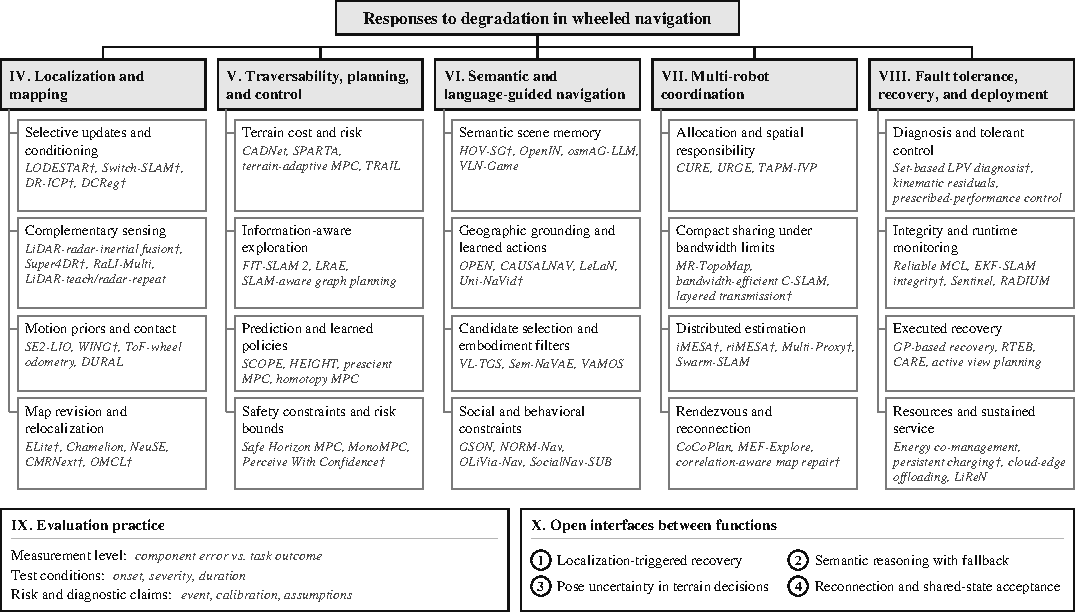
\includegraphics[width=\textwidth]{figures/fig-taxonomy.pdf}
\caption{Organization of the survey. Sections~IV--VIII group responses to degradation by navigation function, with representative methods listed under each response family. The methods are examples rather than complete lists, and $\dagger$ marks examples not evaluated on a wheeled robot or its data. Section~IX compares evaluation practice along three axes, and Section~X examines four interfaces between functions whose behavior under degradation remains insufficiently characterized.}
\label{fig:taxonomy}
\end{figure*}

This survey organizes the literature around three questions: which navigation assumption a degradation affects, how a method changes the information or action available to the robot, and what evidence connects that change to navigation performance. Fig.~\ref{fig:taxonomy} shows the resulting organization by navigation function, response family, and open interface. The main contributions of this survey are summarized as follows. First, this survey compares responses to degradation across five navigation functions together with their sensing, model, and action requirements, distinguishing component improvements from executed recovery. Second, it codes the evaluation evidence of the \CoreCount{} technical publications by navigation function and finds that, in this purposive sample, only \DegTaskShare\% report task outcomes under a named degradation condition. It also examines how platform, reference dependence, computation placement, and experimental design condition the interpretation of reported results. Third, it proposes four interfaces between existing methods that merit joint evaluation and outlines a matched comparison for each, namely localization-triggered recovery, semantic reasoning with fallback, pose uncertainty in terrain decisions, and shared-state acceptance after reconnection.

The remainder of this survey is organized as follows. Section~\ref{sec:background} introduces wheeled motion constraints, the navigation stack, and the sources of degradation, after which Section~\ref{sec:methodology} defines the scope and literature selection. Sections~\ref{sec:localization}--\ref{sec:reliability} develop the technical synthesis, Section~\ref{sec:evaluation} compares evaluation practice, Section~\ref{sec:challenges} presents open challenges, and Section~\ref{sec:conclusion} concludes this survey.

\section{Background}
\label{sec:background}
\subsection{Wheeled Platforms and Motion Constraints}
A wheeled mobile robot moves through driven or steered rolling contacts whose footprint, arrangement, and contact conditions constrain the paths it can execute. Differential-drive robots turn by varying the left and right wheel speeds, skid-steer robots use the same actuation with lateral slip at the contacts, Ackermann vehicles steer the front wheels with a finite minimum turning radius, and omnidirectional platforms generate lateral motion through their wheel arrangement. For a planar reference point with position $(x,y)$ and heading $\psi$, a common idealization is
\begin{equation}
\dot{x}=v\cos\psi,\qquad \dot{y}=v\sin\psi,\qquad \dot{\psi}=\omega,
\label{eq:unicycle}
\end{equation}
where $v$ is longitudinal speed and $\omega$ is angular speed. Under pure rolling, a differential-drive robot with wheel radius $r$, track width $b$, and right and left wheel angular speeds $\omega_R$ and $\omega_L$ satisfies
\begin{equation}
v=\frac{r}{2}(\omega_R+\omega_L),\qquad
\omega=\frac{r}{b}(\omega_R-\omega_L).
\label{eq:differential}
\end{equation}
An ideal bicycle approximation for Ackermann steering instead gives
\begin{equation}
\omega=\frac{v}{L}\tan\delta,
\label{eq:ackermann}
\end{equation}
where $L$ is the wheelbase and $\delta$ is the steering angle. Slip violates the pure-rolling assumption, wheel calibration affects odometry, and steering and acceleration limits constrain tracking. On uneven ground, suspension, pitch, roll, clearance, traction, and payload further affect feasibility, which means that a planar collision-free path may be physically unsuitable even when localization is accurate.

\subsection{The Navigation Stack and Its Degradation}
Fig.~\ref{fig:stack} shows the principal functions of a navigation system, the points at which degradation enters, and the interfaces examined in Section~\ref{sec:challenges}. Cameras, color and depth (RGB-D) cameras, LiDAR, radar, inertial measurement units (IMUs), wheel encoders, global navigation satellite system (GNSS) receivers, and ultra-wideband (UWB) ranging supply measurements with calibration parameters and timestamps. The estimator infers robot state from these measurements and motion inputs, the mapping algorithm estimates spatial structure, the planner selects a route or trajectory, and the controller converts that reference into actuator commands. A supervisor can interrupt execution when measurements, models, or resources no longer support the current action. Deployed systems realize these functions through interacting maps, planners, controllers, and recovery behaviors, for example in a robot operating system (ROS) navigation stack with planner fallback~\cite{P_S16} or under behavior-tree supervision~\cite{P_N17}.

\begin{figure*}[t]
\centering
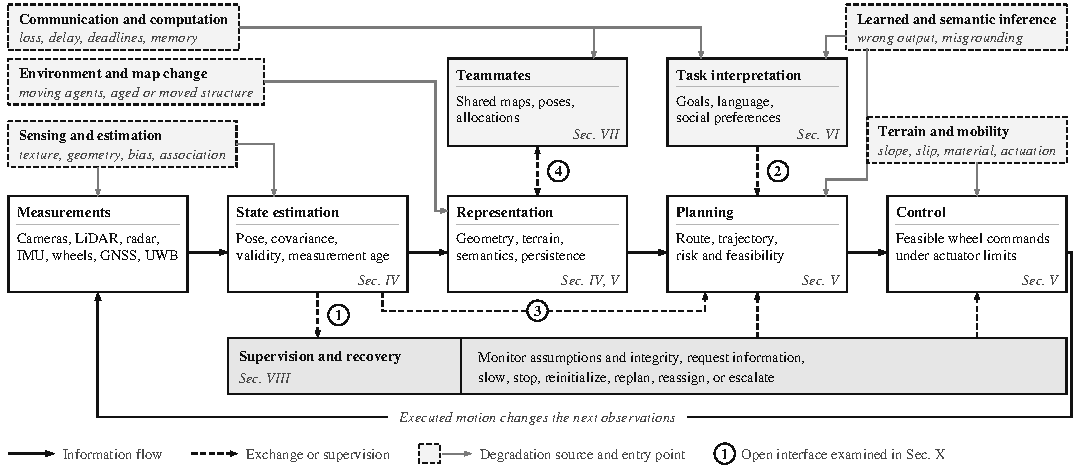
\includegraphics[width=\textwidth]{figures/fig-stack.pdf}
\caption{Navigation functions, degradation entry points, and open interfaces. Each function is colored by the section that reviews it. Teammates and task interpretation supply information to the motion stack rather than bypassing vehicle constraints, and the numbered markers locate the four interfaces of Section~X.}
\label{fig:stack}
\end{figure*}

An estimator can be described through the posterior
\begin{equation}
p(\mathbf{x}_t,\mathcal{M}\mid\mathbf{z}_{1:t},\mathbf{u}_{1:t}),
\label{eq:belief}
\end{equation}
where $\mathbf{x}_t$ is the robot state, $\mathcal{M}$ is the map, and $\mathbf{z}_{1:t}$ and $\mathbf{u}_{1:t}$ denote observation and motion-input sequences available through time $t$. Localization estimates state relative to a given reference, whereas SLAM estimates state and map jointly, commonly through visual--inertial odometry (VIO) or LiDAR--inertial odometry (LIO). ORB-SLAM3~\cite{B_ORBSLAM32021} and FAST-LIO2~\cite{B_FASTLIO22022} are representative visual and LiDAR--inertial systems on which several reviewed methods build. Loop closures constrain revisited places, and an incorrect association can introduce correlated errors into many states. Downstream decisions may therefore require the covariance, association confidence, and age of an estimate as well as its mean. Geometric, topological, and semantic representations retain different information, and a representation sufficient for one decision can be insufficient for another. A place graph may support a long route while omitting a small obstacle, and a terrain label may describe appearance without establishing traction for a loaded vehicle.

In local planning, the dynamic window approach (DWA) searches admissible velocity commands, timed-elastic-band (TEB) optimization adjusts a sequence of poses and timing variables, and model predictive control (MPC) repeatedly solves a finite-horizon control problem. DWA and TEB remain common comparators in recent evaluations~\cite{P_M06,P_M30}. A controller using a control barrier function (CBF) constrains inputs to keep the state within an admissible set under stated assumptions~\cite{P_E24,P_E26}. For a control-affine model $\dot{\mathbf{x}}=f(\mathbf{x})+g(\mathbf{x})\mathbf{u}$, a common condition is
\begin{equation}
\nabla h(\mathbf{x})^{\mathsf T}\bigl[f(\mathbf{x})+g(\mathbf{x})\mathbf{u}\bigr]
+\alpha(h(\mathbf{x}))\geq 0,
\label{eq:cbf}
\end{equation}
where $f$ denotes the drift dynamics, $g$ maps the control input $\mathbf{u}$ to the state derivative, $h(\mathbf{x})\geq0$ defines the admissible set, and $\alpha$ is a suitable increasing function with $\alpha(0)=0$. The resulting safety argument depends on the state information, dynamics, admissible inputs, and update implementation, and penalizing a barrier violation in an objective does not establish the condition during execution.

Here, \emph{degradation} denotes an operating change that reduces the quality or validity of the information, models, resources, or physical capabilities required for navigation. Fig.~\ref{fig:stack} distinguishes four sources that can occur within one episode. Sensing and estimation degradation includes weak texture, illumination change, poorly constrained scan geometry, GNSS denial, timing errors, and incorrect associations, and many measurements may still carry little information along one motion direction. Terrain and mobility degradation includes slopes, vegetation, soft ground, slip, and changed actuator behavior, where similar geometry can hide different friction or sinkage. Environment and map change includes moving people, altered layouts, and construction, which requires the robot to separate transient obstacles from lasting map updates. Communication and computation degradation includes packet loss, partitions, stale shared states, delayed model responses, and missed deadlines, and a restored link raises the further problem of reconciling states accumulated during the outage.

\subsection{Accuracy, Task Performance, and Integrity}
Absolute trajectory error (ATE) measures differences between estimated and reference poses after a declared alignment, relative pose error (RPE) measures motion error over a declared interval, and both are commonly summarized by the root mean square error (RMSE). Their values depend on alignment freedoms, scale treatment, synchronization, aggregation, and the dependence of the reference on the evaluated sensors. Task measures include goal success, collisions, interventions, completion time, coverage, and energy, while success weighted by path length (SPL) combines goal success with path efficiency. Neither task success nor low ATE identifies the source of a failure or the ability to recover after an alarm.

Integrity concerns the risk of an unacceptable estimation error without an adequate warning. A useful conceptual statement is
\begin{equation}
\Pr\!\left(E_t>A_t\ \land\ \text{no timely alert at }t\right),
\label{eq:integrity}
\end{equation}
where $E_t$ is an error magnitude and $A_t$ is an application-specific alert limit. A protection level is an error bound associated with a specified integrity model, and a covariance alone is not a calibrated protection level. Particle-filter and SLAM integrity analyses account for fault hypotheses and association errors when relating alarm conditions to hazardous error~\cite{P_M28,P_X07}. For navigation, the warning must also reach a response policy early enough for the motion and stopping constraints of the robot.

\subsection{Datasets, Simulators, and Transfer}
Table~\ref{tab:benchmarks} relates representative resources to the evidence they can support. M2DGR and M2UD provide ground-robot sequences with sensing and motion difficulties and real-time kinematic (RTK) references~\cite{P_M41,P_F11}, GEODE and HK-MEMS extend the comparison to varied degeneracy and sensor conditions~\cite{P_S33,P_S21}, and robot/network simulation supports repeated reception and control conditions~\cite{P_F13}. Recorded data support reproducible estimator comparisons, although replay does not change future measurements when a planner acts differently. A closed-loop simulator supplies that feedback under its model, whereas hardware adds physical interaction and execution timing, and the three settings answer different causal questions.

\begin{table*}[t]
\centering
\caption{Representative evaluation resources, their intended uses, and relevant limitations.}
\label{tab:benchmarks}
\surveytableformat
\begin{tabularx}{\linewidth}{@{}L{2.8cm}L{5.4cm}Y@{}}
\toprule
\textbf{Resource} & \textbf{Evaluation use} & \textbf{Relevant limitation} \\
\midrule
M2DGR~\cite{P_M41} & Ground-robot localization across everyday sensing and motion difficulties & Estimation errors must be connected separately to task outcomes \\
\addlinespace[3pt]
M2UD~\cite{P_F11} & Uneven-terrain localization/mapping and runtime-aware comparison & References mix RTK and offline SLAM, external checks cover selected routes, and mapping includes handheld capture \\
\addlinespace[3pt]
GEODE~\cite{P_S33} & Degeneracy comparisons across sensor conditions & Sensor-specific coverage and severity affect comparisons, and replay does not test action-dependent recovery \\
\addlinespace[3pt]
HK-MEMS~\cite{P_S21} & Multi-sensor localization and reference comparisons & Missing reference intervals and failed trajectories require explicit coverage reporting \\
\addlinespace[3pt]
Robot/network simulation~\cite{P_F13} & Designed reception and control conditions with repeated trials & A network-in-the-loop simulation is distinct from a distributed physical deployment \\
\bottomrule
\end{tabularx}
\end{table*}

\section{Review Method}
\label{sec:methodology}

This survey covers localization and mapping, traversability and motion control, semantic navigation, multi-robot coordination, and fault management for wheeled mobile robots operating under degraded sensing, terrain, maps, communication, or computation. It includes journal articles and main-conference papers from 2021 to 2026 that propose, evaluate, or benchmark a mechanism for these functions. Studies on road vehicles, other ground robots, or non-ground carriers are included when the inputs of their mechanism exist on a wheeled robot and its assumptions do not rest on the other embodiment. Fig.~\ref{fig:matrix} and Table~\ref{tab:evaluation} count these platform groups separately.

The \CorpusCount{} publications were selected in purposive stages. A language-model-assisted title and abstract screening of robotics journals formed the initial sample, which theme-balanced and targeted searches extended together with works that an internal review of an earlier draft named as missing (Section~\ref{S-supp:selection} of the supplementary material). The corpus is dominated by IEEE publications (\IEEEShare\%) and by works from 2025--2026 (\RecentShare\%). Its counts in Section~\ref{sec:evaluation} therefore describe the selected literature rather than the field. Foundational methods from before 2021 are cited as background outside the coded corpus.

Each work is coded with a published codebook (Section~\ref{S-supp:coding} of the supplementary material). Degradation evidence falls into three classes: a condition injected or varied against a comparator (D1), a condition deliberately selected for its difficulty without manipulation (D2), and an incidental condition that the study reports (D3). A named degradation condition means D1 or D2. A combined attribute such as a task outcome under such a condition counts only when both parts come from the same experiment. A separate language-model session coded a stratified sample of \SampleCount{} works without access to the primary codes, with a median Cohen's kappa of \KappaMedian{} over the double-coded attributes (Section~\ref{S-supp:second-coding} of the supplementary material). This value measures agreement between two language-model coding passes and is not human inter-rater reliability. Reported metrics are interpreted within the platform and protocol of each study, without pooling effect sizes across datasets.

\section{Localization and Mapping}
\label{sec:localization}

Localization and mapping methods respond to degradation through selective measurement updates, complementary sensing, motion priors, relocalization, and map revision. These responses differ in the information they retain and in their assumptions about geometry, contact, and correlations between estimates. Table~\ref{S-tab:localization} in the supplementary material lists representative implementations with their inputs, evaluation settings, and computation placement.

\subsection{Localizability and Selective Measurement Updates}

Geometric degeneracy occurs when measurements constrain some pose directions much less than others. LODESTAR retains information in the weak directions by selecting historical Schmidt--Kalman anchors from the condition of the LiDAR measurement Jacobian and by choosing points according to their contribution along those directions~\cite{P_E01}. With a common FAST-LIO2 backbone, absolute pose error (APE) on the SubT-MRS Long Corridor recording falls from 3.113 to 1.386\,m, while average desktop computation rises from 21.04 to 28.69\,ms. However, the improvement is not uniform, since the APE on the Short exp recording is 0.429\,m against 0.412\,m for the baseline, while the method still requires LiDAR returns. Other detectors characterize degeneracy before acting on it. A screw-theoretic analysis classifies translational, helical, and spherical degeneracy from point, line, range, and bearing constraints~\cite{P_E05}, normal histograms guide feature selection and weighting along weak tunnel directions in DR-ICP~\cite{P_S24}, and a DBSCAN-based detector adapts its decisions from accumulated condition-number history and compensates with IMU motion after a startup phase~\cite{P_S31}. DCReg instead decouples registration and preconditions weak subspaces while preserving the least-squares objective~\cite{P_S37}. Better conditioning exploits weak but nonzero information, although it neither restores an absent constraint nor rescues an initialization outside the convergence basin. Comparisons of selection, compensation, and preconditioning therefore need controls matched to the information that each method exploits.

\subsection{Complementary Sensing}

Complementary sensors supply information that a degraded scan lacks. Switch-SLAM introduces visual constraints when normalized Hessian eigenvalues indicate LiDAR degeneracy and falls back to inertial propagation when both modalities fail~\cite{P_F04}. Degradation-resilient LiDAR--radar--inertial odometry keeps LiDAR constraints along observable directions while radar velocity supplies independent motion information, with flying-robot tests in obscurants~\cite{P_E09}. An equivariant LiDAR--radar--inertial filter instead estimates inertial biases and rejects radar outliers under an exact-map observability assumption~\cite{P_E06}. Radar-centric estimators must also cope with sparse, noisy returns. A continuous-trajectory radar--inertial estimator propagates pose uncertainty to the timestamp of each point and down-weights uninformative points during registration and mapping~\cite{P_R01}, whereas Super4DR learns radar odometry through self-supervision and completes the radar map with Gaussian primitives guided partly by image depth~\cite{P_R12}. RaLI-Multi uses inter-vehicle UWB ranges to correct LiDAR--inertial drift along the detected degenerate direction, assuming at least one well-constrained horizontal direction, while a stopped anchor vehicle optimizes and broadcasts a shared pose graph~\cite{P_R02}. MM-LINS instead hibernates an unreliable map, reinitializes, and later registers overlapping maps~\cite{P_E08}, trading continuous use of one map for recovery through later overlap. Selective updates need surviving geometry, fusion needs measurements that remain informative, and reinitialization needs later overlap, none of which a degeneracy alarm alone establishes.

\subsection{Motion Priors, Contact, and Adaptation}

Ground geometry can enter estimation as a reweighting, a motion prior, or an explicit factor. AESF-LIO adaptively fuses separate ground and non-ground corrections without adding an independent observation~\cite{P_N01}, SE2-LIO parameterizes pose on $SE(2)$ with out-of-plane perturbations modeled as noise~\cite{P_N02}, and a sparse-channel LiDAR system adds a ground-normal factor and intensity features to suppress vertical drift~\cite{P_R03}. Its ground detector misses gradual slope changes, while its indoor references share LiDAR registration with the estimator. These designs address different error causes, although significant slope variation can invalidate the near-planar priors that they share.

Wheel and inertial measurements bridge failures of external sensing when contact and excitation remain adequate. Wheel-aided VIO propagates inertial--wheel motion during visual failure~\cite{P_M24}, PL-VIWO adds motion-consistency rejection and point-assisted line triangulation evaluated on recorded vehicle data with fixed calibration~\cite{P_E10}, and a quadratic motion-manifold estimator integrates wheel measurements on a local ground model that extremely uneven farmland violates~\cite{P_M43}. WING learns corrections for IMU bias and for wheel errors caused by skidding and vertical bouncing on a continuous B-spline ground manifold~\cite{P_R04}. The resulting interoceptive-only odometry serves as a fallback whose benefit depends on how closely the ground follows the manifold. Contact uncertainty can also be estimated explicitly, as when a tire-model observer fuses wheel-level velocity estimates by covariance intersection and excludes inconsistent wheels~\cite{P_M39} or when time-of-flight (ToF)--wheel odometry inflates process covariance only along the remainder that differential-drive motion cannot explain~\cite{P_E02}. DURAL switches between LiDAR--inertial--UWB estimation inside a surveyed anchor region and wheel-aided estimation outside it~\cite{P_E03}. Learned kinematic factors~\cite{P_E04} and the hierarchical modality reweighting of Super Odometry~\cite{P_E07} train motion priors while perception is reliable and freeze them when supervision degrades, which limits the incorporation of unreliable measurements.

Contact and calibration provide additional observations. Lug-generated wheel traces reveal slip on suitable soil~\cite{P_N03}, whereas commanded collisions with known-map geometry constrain pose in a filter, with hardware tests that rely on manually commanded contacts~\cite{P_N19}. GNSS-aided IMU--odometer calibration estimates wheel scale and extrinsics but leaves vertical translation unobservable under planar motion~\cite{P_S32}. Such calibration parameters should not absorb transient contact failure. IL-LIO learns point-to-voxel residuals and uncertainty for nonplanar geometry~\cite{P_S30}, although learned residual variance is not an independently calibrated integrity bound.

\subsection{Dynamic Geometry and Persistent Maps}

Dynamic-scene estimators choose between excluding moving observations and estimating them. Exclusion keeps the static map clean but can remove much of the geometry in crowds, as in semantic rejection of person features in hospital RGB-D SLAM~\cite{P_M44} and in GPU-free asynchronous mask propagation in NGD-SLAM, whose reported tracking time excludes concurrent detection~\cite{P_E19}. DynoSAM instead estimates rigid-object motion in world-centric factor graphs, relying on full-batch optimization without loop closure~\cite{P_E15}. PG-SLAM and JPG-SLAM retain dynamic appearance through Gaussian representations, although neither runs in real time with loop closure~\cite{P_E17,P_E20}. Improved rendering does not by itself establish a better obstacle map. The appropriate representation depends on whether the downstream task needs static geometry or object motion. Dense static maps carry their own cost, as dense multi-scan adjustment fits grid-cell distributions jointly over several scans and runs slower than recording time~\cite{P_N20}.

Across sessions, map maintenance additionally requires an estimate of how long structure persists. ProbPer-LiLo estimates semantic cluster persistence with a survival prior~\cite{P_E16}, ELite weights registration by local and cross-session ephemerality~\cite{P_E18}, and a lifelong LiDAR mapper stores positive and negative map differences from which earlier versions can be reconstructed~\cite{P_E11}. Chamelion learns change detection from synthesized structural changes and separates disappearance from occlusion before updating construction-site and office maps, performing best when registration error and voxel size resemble its training data~\cite{P_R07}. For automotive radar, multi-session loop verification and a temporal occupancy grid retain persistent points for later localization under a planar-trajectory assumption~\cite{P_R09}. NVMS-SLAM keeps normal-bearing surfaces apart to avoid merging opposite faces of thin walls and refines alignment offline~\cite{P_S01}, while NeuSE updates object maps after layout changes within trained categories~\cite{P_S34}. Most of these evaluations use recorded data, handheld acquisition, or injected changes. Map consistency alone therefore does not establish how a moving robot responds to a revised map.

\subsection{Prior-Map and Cross-Modal Localization}

Localization against a compact or structural prior reduces the online representation but becomes sensitive to changes in the mapped environment. ERPoT matches sparse scans to polygon maps after ground removal~\cite{P_M13}, Area Graph localization matches filtered scans to walls and doors with WiFi and barometric initialization~\cite{P_S03}, BIM localization estimates as-designed discrepancies before weighting structural constraints~\cite{P_S36}, and orchard trunk maps suppress seasonal foliage while making global recovery depend on adequate trunk support~\cite{P_S22}. An uncertainty-aware outdoor localizer weights NDT matching by estimated covariance and gates GNSS, a rule that can reject accurate fixes after extended LiDAR loss~\cite{P_M16}. Relocalization obtains new hypotheses from appearance or structure, including cross-attention image retrieval on pushed-robot recordings~\cite{P_M21}, object-level scene graphs that tolerate staged object moves~\cite{P_M34}, distilled LiDAR--camera place recognition~\cite{P_E56}, rendered point-cloud, mesh, or neural-radiance maps~\cite{P_S26}, and density-map loop closure whose maps can inherit front-end degeneracy~\cite{P_S35}. Retrieval provides a candidate rather than a verified pose, which the recovery procedure must then validate.

Cross-modal matching relaxes the requirement that map and query share a sensor. CMRNext casts camera-to-LiDAR matching as optical flow followed by perspective-n-point estimation and transfers across camera setups, although it is trained on driving data, is not yet real time, and receives an initial pose for every frame~\cite{P_R06}. OMCL scores Monte Carlo hypotheses with open-vocabulary features ray-cast from a three-dimensional map and can initialize from a language description, while requiring map-scaled odometry and a static map~\cite{P_R10}. LiDAR Teach, Radar Repeat applies such cross-modal registration within a closed-loop route-repetition system~\cite{P_R11}. Forward-looking 4D radar is localized against LiDAR keyframes from a teaching pass using a Doppler motion prior and an alignment of radar power with LiDAR intensity, and registration errors drive label-free fine-tuning. Route repetition on a four-wheel differential-drive platform covers smoke, moving traffic, and structural change over months, while obstacle avoidance still relies on other sensors.

\subsection{Cooperative Estimates, Uncertain Maps, and Evaluation Resources}

Cooperative estimators add constraints while introducing correlations. CoVOR-SLAM corrects monocular scale with inter-agent ranges in a similarity-pose graph evaluated on recorded data with one stationary rover~\cite{P_F15}, a Lie-group estimator propagates cross-covariances among wheel, inertial, and marker estimates over near-straight indoor motion~\cite{P_E53}, and a fault-tolerant prior-map estimator diagnoses observation, landmark, and odometry faults and lets a repaired landmark benefit a later collaborator~\cite{P_F03}. Uncertainty in the map itself is represented in other ways. Semantic neural processes predict elevation with uncertainty that still requires calibration~\cite{P_S46}, E2-BKI propagates evidential semantic uncertainty through geometry-aligned kernels~\cite{P_R08}, and a multi-fidelity GP explorer weights field samples by localization uncertainty on an aquatic robot~\cite{P_F10}. How a calibrated pose distribution should change wheel-footprint clearance or speed remains open, as discussed in Section~\ref{sec:challenges}.

Benchmarks and active sensing qualify robustness claims. M2DGR and M2UD expose combined sensing and motion difficulties~\cite{P_M41,P_F11}, HK-MEMS and GEODE vary degeneracy, carriers, and reference construction~\cite{P_S21,P_S33}, and robot-mounted lighting in LUCID shows that improved visual appearance does not necessarily improve odometry~\cite{P_S20}. AirSLAM combines learned point and line features with map reuse and reaches 40\,Hz on an embedded GPU under illumination change, although it reduces to a point-feature system where structural lines are absent~\cite{P_R05}.

\subsection{Synthesis}

The main distinction among these methods is which information survives degradation and how the estimator uses it. An estimator can retain constraints in observable directions, add independent motion information from radar, range, wheel, or contact sensing, or bridge weak external sensing with learned or geometric priors whose adaptation is useful only while supervision remains credible. Relocalization and map revision correct accumulated inconsistency through new correspondences, with further requirements for overlap, persistence, cross-modal registration, and correlation handling. Their diagnostics also differ in meaning, since geometric conditioning, motion consistency, and place similarity cannot be treated as a common probability of localization failure.

\section{Traversability, Motion Planning, and Control}
\label{sec:planning}

Motion planning and control connect the estimated environment to executable behavior. Under degradation, feasibility depends on terrain support, obstacle motion, state uncertainty, actuator limits, and the age of control information. The methods below address these dependencies through traversability costs, information-aware exploration, learned prediction and policies, safety constraints, and predictive control, with representative implementations listed in Table~\ref{S-tab:planning} of the supplementary material.

\subsection{Terrain Support and Traversability Costs}

Traversability is a relation between terrain and robot capability, which the reviewed methods express through quantities with different physical meanings. CADNet predicts heading-dependent accessible range from LiDAR history for a TEB planner on a SCOUT robot~\cite{P_M29}, whereas GA-Nav projects attention-based terrain segmentation into a cost map combined with elevation~\cite{P_M40}. A risk-aware learner labels traversed footprints and adds weak obstacle labels before predicting unvisited cells, although its predictions are evaluated only on manually driven recordings~\cite{P_M23}. PE-RRT* infers hidden support planes in vegetation with multivariate Gaussian processes and tracks the route with nonlinear MPC~\cite{P_M26}, while a multilevel planner checks settling, support polygon, and body collision for a tracked robot whose wheeled variant is simulated~\cite{P_M12}. An anisotropic explorer penalizes motion by slope and travel direction with a quasi-static Euler Cost that omits slip and suspension transients~\cite{P_N08}. A footprint label, a support plane, a stability margin, and a cross-slope penalty are not interchangeable estimates of traversal risk. Each is also computed from an estimated pose, and upstream pose error can therefore alter the planning input even when the terrain model is unchanged.

Recent planners condition terrain risk on approach direction and uncertainty and embed it in optimization. SPARTA predicts angle-conditioned risk distributions as reusable Fourier functions from a fully observed prior point cloud~\cite{P_S45}. Its tire-deformation consequences are evaluated in simulation, with a physical demonstration that routes around a virtual risky branch. A visual-foundation-model approach learns cost, speed, and novelty maps from expert driving for MPPI~\cite{P_S42}. In its field trials, operator corrections expose residual failures that offline trajectory agreement conceals. A terrain-adaptive $\epsilon$-constraint MPC minimizes path length while bounding a pose-stability cost adjusted online from terrain descriptors and corrects car-like dynamics with a sparse GP~\cite{P_R13}. Its success falls from 94\% in simulation to 80\% outdoors on a Scout Mini, a drop that the authors attribute to wheel slip and sensor noise, while the planner assumes an offline terrain mesh. TRAIL learns an implicit field of terrain attributes from RGB and LiDAR and optimizes path geometry and speed along its gradients, with field interventions caused by wet-ground traction loss and failures attributed to occlusion and limited field of view~\cite{P_R15}. These systems already make risk-sensitive terrain decisions, whereas map completeness, uncertainty calibration, traction, and physical consequences remain separate evaluation questions.

\subsection{Exploration with Information and Geometry}

Exploration chooses where to improve the map while preserving the ability to localize. FIT-SLAM~2 attaches frontiers to SLAM keyframes, adapts a traversability roadmap after pose changes, and rejects edges with low expected landmark information~\cite{P_E13}. With a common controller and simulator pose, completion takes 880\,s versus 1118\,s for FAEL in Cave but 1809\,s versus 1706\,s in Corridor. Fisher-information evaluation also raises mean planning time from 20.8 to 63.0\,ms. Confidence-rich exploration combines particle-trajectory entropy with occupancy confidence and executes the loop on hardware~\cite{P_E14}, whereas an uncertainty-frontier planner scores coverage with signed relative entropy under known orientation~\cite{P_E12}. Other explorers change the representation of unexplored space, including safety levels for unknown regions in LRAE~\cite{P_M14}, octree category distributions for semantic exploration~\cite{P_M31}, and overlapping free polytopes in FRTree, whose body-containment corridor does not enforce wheeled curvature or rolling-contact limits~\cite{P_M05}. A SLAM-aware planner inserts informative loop closures over a supplied topo-metric graph~\cite{P_N05}. Potential-field MPC integrates frontier and unknown-space costs on a six-wheel skid-steer robot, although without systematic baselines~\cite{P_S02}. The FIT-SLAM~2 results show that more observable routes can cost travel and computation. The benefit of estimation-aware planning further depends on the availability of priors and on useful loop opportunities.

\subsection{Learning, Prediction, and Interaction}

Learning enters planning at different points. NAMR-RRT learns where a risk-aware tree samples~\cite{P_M08}, prescient navigation passes multimodal pedestrian hypotheses to nonlinear MPC that may exhaust its time budget~\cite{P_M30}, and a learned relaxation of optimal reciprocal collision avoidance (ORCA) predicts escape direction and avoidance responsibility~\cite{P_M19}. SCOPE predicts distributions of future occupancy grids from robot motion, tracked objects, and a local static map and inserts their mean and uncertainty into the costmaps of existing planners, with distillation enabling embedded inference~\cite{P_R18}. However, its navigation comparisons are mainly simulated, while its constant-velocity robot model fails during abrupt rotation. Homotopy-driven MPC optimizes distinct trajectory classes in parallel from externally tracked poses~\cite{P_S09}. Candidate diversity reduces local inconsistency without compensating for a missed pedestrian or an incorrect interaction model.

Learned local policies encode observation history implicitly. Visual proximal policy optimization (PPO) adds a motion-perceptibility auxiliary task~\cite{P_M04}, depth-based recurrent PPO is compared with DWA and TEB in simulation~\cite{P_M06}, and a LiDAR actor--critic controller uses spatiotemporal attention under adaptive Monte Carlo localization (AMCL) on a prebuilt map~\cite{P_M22}. HEIGHT separates pedestrians from static obstacles in a heterogeneous spatio-temporal graph and transfers from a low-fidelity simulator to four everyday environments, although its deployed obstacle input assumes a map and reliable localization~\cite{P_R16}. A rough-terrain sim-to-real policy trained with terrain scaling and pose noise still fails under vibration and inaccurate reconstructed geometry, with offboard inference over Wi-Fi~\cite{P_M42}. Lifelong navigation, in turn, learns only where an initial DWA policy supplies useful experience~\cite{P_M45}. As the learned-navigation review notes~\cite{P_X04}, the training data and observation representation determine which disturbances such controllers can accommodate. Recurrence alone therefore does not establish robustness to localization failure.

\subsection{Safety Filters and Explicit Risk Conditions}

A safety filter modifies a nominal command when a constraint would otherwise be violated. A LiDAR-based CBF controller fits a GP to current obstacle edges and uses its mean and gradient in a quadratic program, with an invariance argument that requires known state, unconstrained inputs, and suitable updates while excluding GP variance~\cite{P_E26}. A circulation-embedded CBF adds a tangential constraint and hold logic~\cite{P_E22}, dynamic movement primitives receive a CBF correction to their forcing term~\cite{P_E23}, an adaptive high-order CBF filters iterative LQR commands under input bounds~\cite{P_E24}, a disturbance-estimation CBF compensates matched uncertainty on a tracked robot~\cite{P_E29}, and safe reinforcement learning learns state-dependent high-order barrier penalties alongside soft actor--critic~\cite{P_E30}. Their evidence ranges from external pose and offboard computation to numerical studies. High-order tuning also affects both reaction time and feasibility under actuator bounds.

Other controllers constrain an explicit risk event. A distributionally robust CBF uses noisy barrier samples~\cite{P_M03}, a conditional value at risk (CVaR) controller selects among feasible risk levels in crowds~\cite{P_E27}, and a risk-aware-zone barrier expands an avoidance region under input saturation with a score that is not a calibrated probability~\cite{P_S05}. Safe Horizon MPC samples obstacle trajectories, applies a plan only after slack and support checks, and otherwise decelerates~\cite{P_E25}. In 100 Gaussian eight-pedestrian simulations with a joint-risk specification of 0.05, its mean traversal takes 16.0\,s (standard deviation 1.9\,s) versus 18.4\,s (2.4\,s) for chance-constrained MPC, with maximum estimated plan collision probabilities of 0.0092 and 0.0019. Faster traversal thus accompanies a less conservative plan under the assumed distribution, although the reported probabilities are not empirical collision rates. Perceive With Confidence calibrates obstacle inflation over sampled environments for a planner with an inevitable-collision-set constraint on a legged robot~\cite{P_F08}, whereas conformal crowd navigation limits cumulative intrusion into calibrated pedestrian regions on a Mecanum robot with offboard computation~\cite{P_S48}. MonoMPC learns the distribution of minimum clearance for candidate controls from monocular depth and minimizes a distribution-based risk~\cite{P_R14}. Jackal trials report up to seven times fewer collisions than a navigation stack on the same estimated depth, with planning on a networked laptop and no temporal memory. Chance constraints, CVaR, conformal coverage, and calibrated clearance concern different events. Comparisons should preserve these distinctions rather than read every confidence value as a collision probability.

\subsection{Tracking, Mission Costs, and Network Support}

Tracking control shows how model error, command age, and mission utility enter execution. A GP-MPC controller learns residual dynamics offline from field data and uses only the GP mean~\cite{P_M33}, whereas predictive learning refines repetitive Mecanum trajectories under external UWB pose~\cite{P_M09}. Delay-aware MPC predicts current states from delayed packets and buffers future controls~\cite{P_M27}, whereas vehicle--cloud MPC runs onboard and remote optimizers in parallel and stops on timeout~\cite{P_E21}, two different responses to communication loss. Mission-dependent costs add another reason to change a route, as in infrastructure-based hazard inference added to a cost map~\cite{P_E28} and in payload- or sensing-aware MPPI on a compressed scouting map~\cite{P_X12}. Prescribed-time spatiotemporal tubes assume bounded disturbances and terminal separation without explicit input constraints~\cite{P_N12}, memory-event-triggered MPC reduces repeated solves for a no-slip Ackermann model in hardware-in-the-loop tests~\cite{P_N14}, curvature-constrained vector fields co-design motion and saturation on an Ackermann vehicle with motion capture~\cite{P_S07}, and universal constrained tracking filters references that exceed prescribed state bounds~\cite{P_S08}. Neither a reach-avoid proof without input limits nor fewer solves establishes timely, feasible control on a saturated onboard system.

\subsection{Synthesis}

Motion methods differ in what they change, namely the terrain cost, the sampled route, the predicted occupancy or obstacle motion, or the final command. A terrain cost can favor better support without enforcing stability, whereas a learned policy can avoid familiar interactions without identifying a feasible response to an unseen fault. Explicit constraints make admissibility testable only under their state, dynamics, and update assumptions. The resulting trade-offs concern progress as well as conservatism, and comparisons should therefore establish which of these changes produces the reported task benefit.

\section{Semantic and Language-Guided Navigation}
\label{sec:semantic}

A semantic navigation system that combines task interpretation, scene memory, and motion generation may output a room, an object instance, frontier scores, a path, a cost layer, or an action sequence. The type of output determines how a reasoning error propagates into planning and control. Table~\ref{S-tab:semantic} in the supplementary material lists representative implementations with their sensing and evaluation settings.

\subsection{Semantic Memory and Scene Structure}

Persistent semantic maps support relational queries but must be updated when objects move. HOV-SG organizes a mapped building into floors, rooms, and objects for hierarchical retrieval~\cite{P_E48}, DualMap searches stable anchors globally before checking objects locally~\cite{P_M02}, and OpenIN updates carrier--object existence confidence when an expected object is not observed~\cite{P_E44}. These updates must distinguish removal from occlusion or poor depth, whereas osmAG-LLM assumes from the outset that objects move. It keeps a lightweight text-based area graph for context, asks a language model for likely locations, and confirms targets by online detection~\cite{P_R27}. In 27 of 30 building trials it reaches a correct position, with detection errors causing most failures. Goal-conditioned maps store less reusable structure, as VLFM projects image--language similarity into a frontier value map until a detector supplies the goal~\cite{P_E47}. VLN-Game builds an object-centric three-dimensional map and uses a game-theoretic vision-language model (VLM) to disambiguate attribute-rich descriptions, with quantitative results from Habitat-Matterport scenes~\cite{P_R28}. SysNav reserves VLM calls for room-level decisions and leaves viewpoint selection and waypoint execution to geometric modules~\cite{P_E41}. Multimodal spatial language maps add image and audio features to an offline map, although a remembered sound marks where it was heard rather than its source~\cite{P_S12}. Temporal scene-object graphs report corner trapping and premature termination among their physical failures~\cite{P_S13}. Co-NavGPT extends semantic reasoning to team frontier assignment executed by a geometric policy, with perception and planning on a workstation~\cite{P_N09}.

\subsection{Geographic Grounding, Priors, and Learned Actions}

Outdoor instructions often refer to places beyond the sensor horizon. OPEN associates visual semantics with OpenStreetMap and replans locally when road geometry differs from the map~\cite{P_M10}, G-DRAGON constrains generated identifiers to existing map entities before composing a behavior tree~\cite{P_E46}, and CAUSALNAV retrieves destinations from an object--building--cluster graph and combines global routing with constrained local control~\cite{P_E45}. Their requirements differ in prior exploration, map coverage, heading initialization, and remote computation. Hand-drawn maps and recorded demonstration tours raise similar questions about prior coverage. HAM-Nav associates live landmarks with an imperfect hand-drawn map and predicts omitted ones before A*/TEB execution~\cite{P_S39}, whereas Mobility VLA retrieves a goal frame from a demonstration tour and routes over an offline graph without exploring~\cite{P_S43}.

Learned policies map language and images directly to motion, as in LeLaN, which trains a last-mile policy from labeled robot and action-free video~\cite{P_E50}. In 150 trials with 28 initially visible objects, its success within 0.2\,m is 0.89 versus 0.67 for OWL-v2 with ZoeDepth, while a separate 15-trial ablation reaches 0.60 arrival with collision training and 0.13 without it. These results separate target grounding from obstacle handling without establishing open-world search or a collision-risk bound. Uni-NaVid compresses multiscale video history before predicting discrete primitives whose vocabulary bounds the available actions~\cite{P_E49}. LGX instead prompts a language model for exploration directions and falls back to random exploration after an invalid response~\cite{P_M20}.

\subsection{Candidate Selection and Behavioral Constraints}

Selecting among explicit candidates confines semantic errors to a choice among feasible alternatives. VL-TGS generates LiDAR-based trajectories, projects them into an image for GPT-4V ranking, and follows the choice with DWA while later decisions are pending~\cite{P_F05}. However, its ranking cannot recover a route that the generator never proposes. Sem-NaVAE applies the same generate-and-select structure without a map, scoring conditional-VAE proposals with lightweight open-vocabulary segmentation and reporting 90\% success on 120--240\,m campus and park routes with few repetitions per route~\cite{P_R25}. VAMOS adds an embodiment filter, in which a per-robot affordance model trained in simulation re-ranks the image-space paths proposed by a VLM planner~\cite{P_R26}. With the planner unchanged, the affordance model of a wheeled robot raises its success on a ramp-or-stairs task from 60\% to 90\%, a gain indicating that semantic proposals need filtering by the capabilities of the executing chassis.

Social and behavioral constraints separate preference from collision geometry. VLM-Social-Nav converts cue-triggered judgments into social costs for DWA~\cite{P_M07}, VLM-informed path selection ranks clustered detours before an ORCA controller computes velocities~\cite{P_E43}, and GSON supplies group labels to a mid-level planner above a barrier-constrained predictive controller~\cite{P_F06}. NORM-Nav parses free-form instructions with a language model and writes semantic, directional, and speed layers into costmaps for standard grid planners, with quantitative comparisons in simulation~\cite{P_R30}. OLiVia-Nav distills large-model social reasoning into lightweight encoders that are updated online and is evaluated against expert trajectories and personal-space violation rather than collision rates~\cite{P_R29}. Safe-VLN masks predicted waypoints with simulated occupancy and selects a new waypoint after a collision occurs~\cite{P_M18}. SocialNav-SUB tests the reasoning premise directly, showing that strong VLMs still trail human consensus and position-based rules on social scene questions~\cite{P_S44}. Physical feedback can ground semantic terrain estimates, as VLM-GroNav revises terrain costs and waypoints from visual and proprioceptive exemplars while depending on GPS and a cloud API~\cite{P_S40}. A grouping or grounding error can thus alter the route even when the local controller avoids detected people, whereas an occluded pedestrian can invalidate the controller itself.

\subsection{Memory, Timing, and Embodied Execution}

Semantic decisions remain valid for different durations. TARIC triangulates intermittent goal cues into a particle memory whose dispersion limits heading deviation during cue-free travel~\cite{P_E42}. SysNav queries at room transitions, GSON uses updated keyframes, and the social path selector associates asynchronous responses with current candidates~\cite{P_E41,P_F06,P_E43}, whereas VAMOS plans at 1\,Hz on a laptop GPU~\cite{P_R26} and OLiVia-Nav moves reasoning into compact encoders~\cite{P_R29}. A room decision can outlive a pedestrian detour, and response age must therefore be judged against the referenced scene. A fast local controller, in turn, can absorb a slow query only while it retains a valid action. Embodiment then determines how a semantic choice becomes motion. VLFM uses different low-level controllers in simulation and on Spot~\cite{P_E47}, Uni-NaVid runs remote inference on a quadruped~\cite{P_E49}, and LeLaN executes on a wheeled base~\cite{P_E50}. For wheels, turning in place, lateral motion, and reversing are available only if the chassis supports them. Map or tour preparation, cloud availability, and the actions available during pending inference also belong in the comparison~\cite{P_S12,P_S43,P_S39}.

\subsection{Synthesis}
\label{sec:semantic-synthesis}

The reviewed systems connect semantic reasoning to motion through scene memory, geographic grounding, learned actions, cost layers, or candidate selection. Persistent maps support reuse but require validity updates, direct policies depend on their history and action vocabulary, and candidate-based systems remain limited by the generator, the embodiment filter, and the local controller. Semantic correctness and collision avoidance therefore require separate evaluation. Matched trials with incorrect or delayed inference can then establish how rejection and fallback affect completion, collisions, and resource use.

\section{Multi-Robot Coordination}
\label{sec:multi}

Multi-robot coordination involves task allocation, information exchange, state fusion, and motion interaction. Since teams exchange frontiers, maps, observations, poses, or position histories, communication degradation turns local operation and shared-state consistency into separate objectives. Table~\ref{S-tab:multi-robot} in the supplementary material lists representative mechanisms with their evaluation settings.

\subsection{Task Allocation and Spatial Responsibility}

Allocation reduces redundant work through a common state. Centralized planners partition merged maps into dynamic Voronoi cells in CURE~\cite{P_M17}, assign known targets over a sparse Delaunay graph with priority yielding in DMT-CPP~\cite{P_E35}, or assign tasks before the mission while penalizing capability shortfall~\cite{P_M32}. Distributed methods reduce negotiation without removing shared state. CQLite exchanges selected Q-values and frontiers~\cite{P_M25}, LPFE predicts teammates' frontier choices from a common map and last known positions~\cite{P_E34}, and 4CNet predicts map structure from shared trajectories with an estimated confidence~\cite{P_E33}. Such inference avoids messages only while robots hold compatible inputs. URGE abstracts the map into subregions with exploration states and allocates them by jointly minimizing path cost and balancing load~\cite{P_R22}. Its full-set exchange with an explored-overrides-unexplored rule lets regional maps converge after a link returns. Its baseline comparisons assume ideal communication in simulation, whereas three-robot runs in a forest, a parking lot, and a tunnel use an ad hoc mesh network. Terrain-aware partitioning (TAPM-IVP) extends spatial responsibility to uneven ground with communication-radius-constrained regions and traversability-aware subgoals~\cite{P_F09}. In ten simulated trials of Scene~1, each robot succeeds in 90\% of trials, compared with 40\% and 30\% for an ablation that removes both partitioning and greedy subgoal selection. These per-robot rates do not give the probability that the whole team completes the mission. The plane-fitting covariance, moreover, describes terrain scatter rather than propagated pose uncertainty.

\subsection{Compact Sharing and Distributed Estimation}

Compact representations trade bandwidth against what teammates can infer. MR-TopoMap shares topological vertices with place descriptors while keeping local occupancy for avoidance~\cite{P_M36}, Cross-rank exchanges position histories and assigns directions at intersections~\cite{P_F14}, and WiSER-X infers relative positions from radio pings that require an interpretation when they are missing~\cite{P_E32}. SlideSLAM buffers exchanged object observations until a loop closure fixes the frame transform~\cite{P_E31}, whereas Commerge minimizes transmitted scans for central submap registration without adapting to radio capacity~\cite{P_E36}. Bandwidth-efficient collaborative SLAM separates lossy mutual-information keyframe selection from lossless entropy coding under a central back end~\cite{P_S29}. Feedback-guided hierarchical transmission sends a pose-and-factor skeleton, prioritized geometry, and semantic labels in layers and reallocates bandwidth each round from back-end loop-closure and risk signals~\cite{P_R21}. However, its dataset-replay evaluation reports estimated rather than measured collision risk, while the authors note that round-wise guidance can become stale under asynchronous links. PROMO-Orchard gates submap merging with orchard priors and posterior checks against a reference built by the same backbone~\cite{P_S23}.

Distributed estimators must also handle delayed and repeated information. iMESA keeps local incremental factor graphs and updates consensus variables through a two-stage exchange that must complete once started~\cite{P_E40}. riMESA, a direct extension by the same authors, removes this blocking requirement~\cite{P_R23}. It formulates collaborative SLAM as edge-based consensus ADMM, rejects outliers with a robust local solver, and discards failed exchanges, with experiments that replay recorded LiDAR factors under Wi-Fi or radio connectivity models. Multi-Proxy combines lightweight descriptors for progressive loop detection with asynchronous ADMM pose-graph optimization~\cite{P_R20}. Under simulated packet loss and latency, a two-stage Gauss--Seidel baseline fails to converge while Multi-Proxy continues, although the method relies on stable front-end odometry. Parallel graph inference separates current-state from historical-message inference~\cite{P_E37}, whereas CoVOR-SLAM shares poses, covariances, and ranges instead of features~\cite{P_F15}. Swarm-SLAM runs decentralized inference with sparse loop prioritization online on a heterogeneous physical team~\cite{P_S10}, whereas foundation-model loop closing anchors monocular scale with metric odometry in Jetson replay~\cite{P_S11}. Radio geometry adds constraints with their own assumptions, as in cooperative range-only SLAM analyzed offline with all landmarks visible~\cite{P_S27} and formation-controlled UWB anchors whose geometry competes with obstacle clearance~\cite{P_S28}. A prior-graph extension adds informative loop edges to multi-robot coverage paths~\cite{P_N07}, building on single-robot SLAM-aware planning~\cite{P_N05}, although its approximation bound concerns the graph objective rather than physical loop correspondences.

\subsection{Rendezvous, Disconnection, and Conditional Repair}

Communication can become part of the motion objective. A rendezvous-aware explorer creates backtracking frontiers from decaying trajectory records~\cite{P_E38}, whereas a communication-constrained controller schedules sub-team meetings that require full-team agreement to update~\cite{P_E39}. CoCoPlan treats team-wise communication events as decision variables and co-optimizes them with task assignment through branch-and-bound search~\cite{P_R19}. In simulations with up to 100 robots, it reports a 22.4\% higher task-completion rate and 58.6\% lower communication overhead than the compared protocols. MEF-Explore derives rendezvous from entropy fields while assuming that low-rate position exchange is always available~\cite{P_R24}. With three TurtleBot2 robots, it explores 21.32\% faster with a 16.67\% higher success rate than the baseline. All of these methods depend on reaching an encounter, exchanging the required state, and executing the subsequent plan.

During disconnection, robots can continue locally and reconcile later. ROAM continues planning from local maps during observed Wi-Fi cutoffs at the cost of revisits~\cite{P_X08}. Correlation-aware collaboration exchanges states, covariances, and cross-covariances of common landmarks before Kullback--Leibler averaging and Schmidt--Kalman updates, a procedure that excludes faulty observations and corrects uncertain landmarks~\cite{P_F03}. Failure-aware target tracking fuses target estimates by covariance intersection after reconnection and lets a permanently isolated drone signal a hazard~\cite{P_F12}. The communication-aware CBF controller relaxes conflicting constraints and drops unreliable links, with recovery evaluated under partial connectivity~\cite{P_F13}. Planned synchronization makes observation an action, scheduling check-ins in which a TurtleBot pair stops and pans to observe each other~\cite{P_S25}. A range-based integrity monitor reconstructs shared localization errors with distributed ADMM, although its demonstration runs centrally on emulated ranges~\cite{P_N11}. These mechanisms address target estimates, landmarks, links, or observations, although none of them supplies a complete protocol for accepting stale or biased map content after an uncontrolled partition.

\subsection{Motion Interaction and Persistent Service}

Coordination also occurs below the allocation layer. RL-RVO learns a distributed velocity policy from reciprocal velocity-obstacle features with external localization~\cite{P_M38}, predefined-time formation control compensates modeled actuator faults over a fixed graph~\cite{P_X13}, and compensation-based MPC estimates model discrepancy online for four motion-captured nonholonomic robots, leaving deadlock to future work~\cite{P_R17}. Reachability-based platoon control preserves separation under bounded inputs while assuming reliable communication~\cite{P_S04}, whereas distributed barrier control adds a coordinated deadlock response on physical vehicles~\cite{P_S06}. In mEclares, a scheduler reserves return and landing opportunities from energy and timing conditions, with agents falling back to committed paths after disconnection~\cite{P_E57}. These results establish implemented coordination responses, whereas degraded-network validity requires its own fault model and trials.

\subsection{Synthesis}
\label{sec:multi-synthesis}

Coordination methods reduce redundant work through allocation, compact representations, or distributed inference. Lower message volume changes which information is available without resolving inconsistencies between local estimates. Rendezvous planning, asynchronous optimization, and local planning sustain activity during disconnection, whereas reconnection additionally requires validating correspondences, accounting for correlations, and deciding which updates to accept. Evaluations with moving wheeled teams should therefore relate communication loss and reconnection to estimate divergence, coverage, interventions, and recovery time.

\section{Fault Tolerance, Recovery, and Long-Term Deployment}
\label{sec:reliability}

Fault detection, isolation, accommodation, and restoration need not occur together, since a controller may tolerate bias of unknown source (Table~\ref{S-tab:reliability} in the supplementary material).

\subsection{Fault Estimation and Tolerant Control}

Analytic redundancy provides diagnosis without duplicating every sensor. Kinematics-based detection compares position, angular velocity, and acceleration through transport relations, with faults injected into recorded rover data~\cite{P_E51}. A linear parameter-varying (LPV) vehicle diagnoser combines zonotopic set-membership estimation with invariant-set bounds, in which separation from the healthy set establishes detectability and overlap between fault classes prevents unique isolation~\cite{P_N16}. Tolerant controllers instead accommodate faults in specified channels, each relying on a different remaining capability. Mixed-gain prescribed-performance control tolerates partial wheel-effectiveness loss~\cite{P_M15}, whereas virtual-error control tolerates heading and wheel-speed faults but assumes exact position~\cite{P_M01}. Adaptive sliding-mode control handles injected actuator faults and saturation on industrial hardware as long as some actuation remains~\cite{P_E52}, while fixed-time adaptive tracking accommodates dead zones and modeled actuator faults in MATLAB studies~\cite{P_S15}. An observer-based event-triggered controller reconstructs modeled faults before issuing updates in hardware-in-the-loop tests of a low-speed, no-slip vehicle~\cite{P_F02}.

\subsection{Integrity and Failure Monitoring}

Monitors differ in the failure event they characterize. Reliable Monte Carlo localization (MCL) estimates a latent localization-success state alongside pose and triggers free-space global relocalization~\cite{P_M35}. Integrity analysis for extended Kalman filter (EKF) SLAM accumulates landmark fault risk into the integrity risk \eqref{eq:integrity}~\cite{P_X07}. In its recorded example, this risk crosses the threshold only after localization fails. A prior-line-map protection level predicts estimation error, with operational alerting left for future work~\cite{P_F01}. Monitors of learned policies use statistical alarm definitions, as conformal anomaly detection controls the nominal false-alarm rate under exchangeability~\cite{P_E54}, while Sentinel pairs fast action-consistency monitoring with slower vision-language progress assessment~\cite{P_F07}. PAAD predicts anomalies along a planned path on field recordings in which people reposition the robot after failures~\cite{P_N18}. RADIUM moves failure prediction before deployment by sampling environment parameters from a distribution conditioned on failure and repairs the policy on the discovered cases, reporting up to five times higher robustness for a repaired vision-in-the-loop policy on a 1/10-scale car~\cite{P_R36}.

\subsection{From Diagnosis to an Executed Response}

The response must match the location of the fault in the stack. In the estimator, fault-tolerant prior-map collaboration excludes faulty observations, inflates faulty-landmark covariance, and specifies reinitialization for odometry faults without evaluating an executed reset~\cite{P_F03}. At the planning level, a GP predictor of safe-corridor optimizer failure triggers a stop--reposition--resume sequence~\cite{P_E59}. With the same planner in simulation, recovery yields eight successes in ten runs against three in ten in a dense world with 1\,m doorways, whereas both variants succeed in all ten runs in a sparse world with 2\,m doorways. However, the predictor posterior concerns planner failure rather than collision. At the level of the controller and supervisor, a fault-aware CBF controller optimizes over candidate sensor or actuator fault sets in numerical examples~\cite{P_E55}, whereas FORTRESS caches slow semantic reasoning for runtime reach-avoid fallback on a quadrotor~\cite{P_E60}.

Implemented recovery policies differ in what they restore, from localization to task feasibility. A nonlinear MPC (NMPC) visual navigation system stops after tracking loss and attempts relocalization~\cite{P_N10}, whereas behavior-tree supervision on CENTAURO chooses among contact repositioning, reversing, replanning, and human assistance~\cite{P_N17}. Task-level policies change the mission instead, as resilient temporal-logic planning relaxes task windows or removes tasks when local correction fails~\cite{P_N15} and predictive swarm fault tolerance withdraws an affected robot to maintenance before complete failure~\cite{P_N13}. Local recovery acts on the trajectory or the observations, through hybrid-A* reinitialization of an infeasible local trajectory in RTEB~\cite{P_S16}, return toward familiar visual states in SCALE~\cite{P_S38}, and repulsive corrections from estimated depth to a visual policy in CARE~\cite{P_S47}. However, neither familiarity nor estimated depth supplies a clearance certificate. Help Me Through learns viewpoint actions from about 50\,h of human demonstrations, or 20\,h followed by online fine-tuning, to keep monocular SLAM tracking through texture-poor transitions, with a physical test that runs the policy on live images while a person teleoperates path planning~\cite{P_R33}. When a robot cannot restore a capability, the team can reassign its task, as in energy-aware allocation under staged capability loss on Robotarium~\cite{P_S17} and in R-FAC, whose log-sum-exp value factorization keeps search policies effective when members fail without notification, assuming perfect target detection~\cite{P_R35}.

\subsection{Resources and Sustained Operation}

Resource choices determine whether a response remains available. CODEI selects bodies, sensors, algorithms, and computing units from catalogs by coupling simulated planner queries to characterized perception errors~\cite{P_M11}. Joint runtime control of motor speed and processor voltage and frequency on a wheeled rover reduces total energy by up to 36.34\% relative to prior methods, with measurements showing that computation can dominate the energy of slow motion~\cite{P_R32}. Fleet availability adds charging constraints, as in cyclic scheduling of operating and charging periods under a station budget~\cite{P_E58} and in persistent-monitoring routes that minimize team size under revisit-latency and recharging limits with deterministic discharge~\cite{P_R34}. A ten-home assistive deployment combines docking rules, cloud orchestration, and remote supervision, with internet problems and localization failures among the causes of interruption~\cite{P_M37}. A cloud--edge system offloads mapping and trajectory generation over 5G while keeping MPC tracking and collision avoidance on Jetson-equipped Ackermann robots, falling back to a leader-based local network~\cite{P_R31}.

Maintenance and learning form a second operational loop. Predictive data acquisition selects new training observations for teach-repeat-learn navigation from visual matching ambiguity~\cite{P_N06}. SELFI stabilizes deployment-time reinforcement learning with a model-based objective and counts interventions during learning~\cite{P_S14}, while LiReN combines foundation-model adaptation with pseudo-resets, keepout rules, charging, and help escalation~\cite{P_S41}. Counterfactual replay selects among adapting policies at the cost of between-trial computation~\cite{P_S18}.

\subsection{Synthesis}

Recovery quality in long-term service concerns both restored operation and the interruptions needed to achieve it, which depend on charging, energy, network access, offboard computation, and human assistance. The studies reviewed here contain \RelIntegrityCount{} of the \IntegrityCount{} integrity or failure-risk assessments in the sample (Table~\ref{tab:evaluation}), mostly with injected or simulated faults.

\section{Evaluation Practice}
\label{sec:evaluation}

\begin{table*}[t]
\centering
\caption{Responses to degradation by navigation function, the conditions under which they help, and the main evidence gaps, with representative studies.}
\label{tab:synthesis}
\surveytableformat
\begin{tabularx}{\linewidth}{@{}L{2.35cm}YYY@{}}
\toprule
\textbf{Function} & \textbf{Main responses} & \textbf{Conditions for benefit} & \textbf{Main evidence gaps} \\
\midrule
Localization and mapping (Sec.~\ref{sec:localization}) & Selective updates, complementary sensing, motion and contact priors, relocalization, map revision~\cite{P_E01,P_F04,P_E02} & Surviving observable geometry, independent measurements, credible supervision for learned priors, later overlap~\cite{P_S37,P_E07,P_E08} & Mostly recorded or replayed data. Degeneracy and similarity scores differ in meaning. Revised maps rarely drive executed responses~\cite{P_K01,P_R07} \\
\addlinespace[3pt]
Traversability, planning, and control (Sec.~\ref{sec:planning}) & Terrain costs, information-aware exploration, learned prediction, safety filters and risk constraints, delay-aware tracking~\cite{P_K03,P_E13,P_E26} & Accurate pose and terrain coverage, priors and loop opportunities, training coverage, known state and admissible inputs~\cite{P_S45,P_N05,P_M42} & Estimated rather than measured collision risk. Few simulation-to-hardware comparisons. Pose uncertainty rarely propagated into terrain decisions, its effect untested~\cite{P_E25,P_K05} \\
\addlinespace[3pt]
Semantic navigation (Sec.~\ref{sec:semantic}) & Semantic memory, geographic grounding, learned actions, language-derived cost layers, candidate selection with embodiment filters~\cite{P_E44,P_M10,P_R26} & Valid map updates, coverage of prior maps or tours, feasible proposed candidates, a local controller valid during pending inference~\cite{P_S43,P_F05} & Incorrect or stale reasoning rarely injected. GPS, cloud, and map-preparation dependencies. Few physical trials per route~\cite{P_S44,P_S40,P_R25} \\
\addlinespace[3pt]
Multi-robot coordination (Sec.~\ref{sec:multi}) & Allocation and spatial partition, compact sharing, distributed and asynchronous estimation, rendezvous, estimate repair after reconnection~\cite{P_R22,P_R21,P_R19} & Compatible shared inputs, reachable encounters, stable front-end odometry, tracked correlations~\cite{P_E34,P_R20,P_F03} & Mostly ideal or modeled communication. Acceptance of stale or biased content after a partition untested on moving teams~\cite{P_R23,P_K07} \\
\addlinespace[3pt]
Fault tolerance and recovery (Sec.~\ref{sec:reliability}) & Analytic redundancy and tolerant control, integrity and runtime monitoring, executed recovery, resource and service management~\cite{P_E51,P_X07,P_E59,P_R32} & A modeled fault channel with remaining actuation, a monitored event that matches the response, trustworthy state for the recovery maneuver~\cite{P_E52,P_M35} & Injected or simulated faults. Restarted or censored trials. Interruptions and human assistance seldom reported~\cite{P_E55,P_N10,P_N17} \\
\bottomrule
\end{tabularx}
\end{table*}

Since most evidence gaps in Table~\ref{tab:synthesis}, which draws Sections~\ref{sec:localization}--\ref{sec:reliability} together, concern how a result was evaluated rather than whether a mechanism exists, this section compares evaluation practice across the reviewed functions.

Evaluation of autonomy under degradation must relate component outputs to executed behavior. The comparison below follows three axes, namely the level at which performance is measured, the conditions under which degradation is tested, and the event and assumptions behind a risk or diagnostic claim. Fig.~\ref{fig:evaluation} connects the three axes through one time-aligned navigation episode with a degraded interval. Table~\ref{tab:evaluation} counts the coded attributes among the \CoreCount{} technical publications for each reviewed function.

\begin{table}[!ht]
\centering
\caption{Reported evaluation attributes among the \CoreCount{} technical publications. Attributes overlap; context publications are excluded.}
\label{tab:evaluation}
\surveytableformat
\begin{tabularx}{\linewidth}{@{}Yr@{}}
\toprule
\textbf{Attribute} & \textbf{Publications} \\
\midrule
\textit{Measurement level} & \\
Component measures & 160 \\
Task outcomes & 128 \\
\addlinespace[3pt]
\textit{Test conditions} & \\
Degradation testing & 130 \\
\addlinespace[3pt]
\textit{Risk and diagnostic assessment} & \\
Integrity/reliability & 14 \\
\bottomrule
\end{tabularx}
\end{table}


\subsection{Measurement, Test Conditions, and Claim Interpretation}

\emph{Component measures} include trajectory, mapping, segmentation, prediction, and tracking error together with runtime and classification scores, whereas \emph{task outcomes} concern completion, collision, coverage, traversal time, intervention, and service availability. \emph{Degradation evidence} describes an experimental condition rather than a metric, in classes of Section~\ref{sec:methodology} that range from injected faults, outages, or varied terrain against a comparator (D1) to difficult sequences, sites, or crowds selected without manipulation (D2) and incidental conditions (D3). A matched nominal control is a stricter variant of D1, used below as a sensitivity definition. For \emph{risk and diagnostic assessment}, the defined event matters, since classifier recall, nominal false-positive control, protection-level coverage, and undetected hazardous error are not interchangeable, as reliable MCL, conformal anomaly detection, and EKF-SLAM integrity illustrate~\cite{P_M35,P_E54,P_X07}.

\subsection{Evidence Across Navigation Functions}

The counts in Table~\ref{tab:evaluation} describe the selected sample rather than the field, and assessment depth varies as disclosed in the supplementary material. Three patterns are nevertheless large enough to qualify the comparisons of Sections~\ref{sec:localization}--\ref{sec:reliability}. First, evidence for localization and mapping stops at the estimate, since all \LocTechCount{} studies report component measures and \LocNamedCount{} name a degradation condition, whereas only \LocTaskCount{} reports a task outcome. Planning and semantic studies show the opposite profile, with task outcomes in \PlnTaskCount{} of \PlnTechCount{} and \SemTaskCount{} of \SemTechCount{} studies. Second, \DegTaskCount{} publications (\DegTaskShare\%) report a task outcome under a named degradation condition in the same experiment, the combination that ties a degraded condition to executed behavior. The share rises from \LocSameShare\% in localization through \MrcSameShare\% in multi-robot coordination, \RelSameShare\% in fault management, and \SemSameShare\% in semantic navigation to \PlnSameShare\% in planning and control. Of these publications, \DOneSameCount{} rest on a condition injected or varied against a comparator and \PhysSameCount{} on a physical robot. Third, the sample contains only \IntegrityCount{} publications with integrity or failure-risk assessment and \ComputeUnreported{} publications that do not report computation placement.

These shares are statistics of the purposively selected sample that depend on definitions and subsets (Table~\ref{S-tab:sensitivity} in the supplementary material). The headline share falls to \DOneNominalShare\% when the condition must be varied against a nominal level, becomes \AnyUnitShare\% when the two attributes may come from different experiments, and was \DegTaskShareCard\% under the card-level coding of an earlier draft. It is \DepthFullShare\%, \DepthLegacyShare\%, and \DepthTargetedShare\% among full, earlier-extraction, and targeted readings, and \WhlShare\% among target wheeled robots against \NonWhlShare\% among other carriers. The share stays between \StageMinShare\% and \StageMaxShare\% when any one selection stage is removed, at \QuotaShare\% in the quota stages against \NonQuotaShare\% elsewhere, and between \YearMinShare\% and \YearMaxShare\% across year bands. In every stage, depth, and quota subset, localization keeps the lowest or a tied lowest share and planning the highest.

\subsection{Execution and Reference Dependence}

\begin{figure*}[!t]
\centering
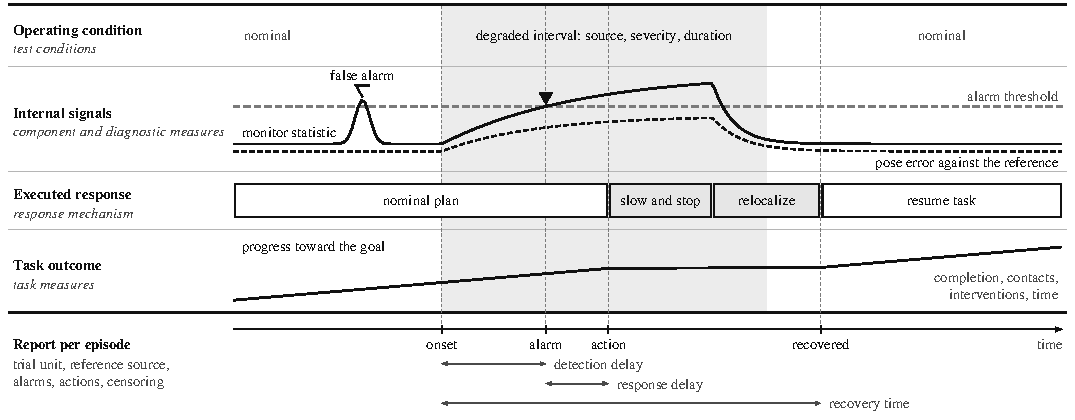
\includegraphics[width=\textwidth]{figures/fig-evaluation.pdf}
\caption{Joint evaluation of detection and response in one navigation episode. The shaded band marks the degraded interval. The operating condition defines the test, internal signals carry component and diagnostic measures, and the executed response and task outcome carry task measures. Detection delay, response delay, and recovery time follow from the synchronized events. A threshold crossing while the pose error stays below the alert limit counts as a false alarm, and an error above the alert limit without a crossing counts as a missed detection.}
\label{fig:evaluation}
\end{figure*}

Recorded measurements preserve sensor artifacts without testing feedback between the estimated state and future observations, whereas closed-loop evaluation lets the evaluated output change the commands and thus the subsequent observations. External pose, offboard processing, teleoperated prior mapping, and staged scenes define the conditions of that feedback, as when slip-aware fusion runs without a controller consuming its estimates~\cite{P_M39} and LiDAR-based barrier control runs under external pose and offboard computation~\cite{P_E26}.

References introduce their own dependence when they share sensors or processing with the evaluated method, as in campus line localization~\cite{P_F01}, kinematic diagnosis with a substitute position~\cite{P_E51}, and orchard map merging scored against its own mapping backbone~\cite{P_S23}. Reference quality also varies within datasets, through the mix of smoothed RTK, offline multisensor SLAM, and selected laser-tracker checks in M2UD~\cite{P_F11}, the untimestamped HK-MEMS bus-route reference~\cite{P_S21}, and scene-dependent reference construction in GEODE~\cite{P_S33}. Cooperative range-only SLAM runs offline on joystick-recorded bags~\cite{P_S27}, whereas hierarchical map transmission reports an estimated risk field from dataset replay rather than measured contacts~\cite{P_R21}. Controlled variables must also match the claimed mechanism. Varying terrain geometry tests plane-fitting allocation~\cite{P_F09}, whereas a test of pose-aware terrain decisions must vary pose uncertainty. Similarly, communication studies rank methods under ideal simulated links in URGE~\cite{P_R22} and replay benchmark factors under modeled connectivity in riMESA~\cite{P_R23}, two settings that do not measure how physical link loss changes the ranking.

\subsection{Guarantees, Rates, and Denominators}

A formal safety result applies to a specified event, probability space, horizon, and set of assumptions. A scenario-planning certificate concerns the risk of an accepted plan under a predicted obstacle distribution~\cite{P_E25}, while environment-level perception calibration depends on representative calibration environments and known state~\cite{P_F08}. A barrier proof may assume feasible inputs for \eqref{eq:cbf} that saturation violates~\cite{P_E26}. Spatiotemporal-tube guarantees likewise assume bounded disturbances and terminal separation without explicit input limits~\cite{P_N12}. None of these guarantees is an empirical closed-loop collision frequency, which must be estimated from executed trials.

Empirical rates require a denominator and an independent trial unit. Across ten homes, the assistive-robot study records 1539 service requests, of which 1130 succeeded, 177 failed, and 232 were not performed~\cite{P_M37}. Its 86.46\% success rate uses the 1307 attempted interventions as denominator and is therefore not the fraction of requests served. Eligibility and censoring change the represented population. Some studies remove scenarios before reporting, as when the CENTAURO study discards infeasible or slowly planned scenarios~\cite{P_N17}. Others remove methods or runs after a failure, as cross-modal teach-and-repeat excludes methods that fail on the first route from later routes~\cite{P_R11}, an outdoor visual-inertial benchmark averages error only over surviving runs~\cite{P_S19}, and multi-session radar mapping omits failed baselines from its averages~\cite{P_R09}. A trial repeated after failed relocalization~\cite{P_N10} differs from recovery within the original attempt. Completion after temporal-logic relaxation~\cite{P_N15} must likewise name the requirements that were changed. Safety and completion must also be reported together, since refusing every action reduces collisions while preventing useful work.

\subsection{Timing, Placement, and Comparisons}

Timing should cover sensing age, transport, perception, estimation, planning, supervision, command delivery, and actuator response, which processor identity and average module runtime do not establish. Fast and slow monitors~\cite{P_F07}, cached reasoning~\cite{P_E60}, slow VLM planning~\cite{P_R26}, and change detection at 2.74\,Hz on an embedded GPU~\cite{P_R07} each need a local controller that stays valid between outputs. DMSA processes data at 1.5--4 times the recording duration and distinguishes unsupported sensor adaptations from failed runs~\cite{P_N20}. Memory-event-triggered MPC counts updates on an industrial computer rather than measuring onboard execution~\cite{P_N14}. A study of LiDAR--inertial non-reproducibility repeats each experiment 30 times after controlling subscribers and buffering~\cite{P_N04}, showing that repeated playback characterizes implementation variability rather than variation across missions.

\begin{table}[!t]
\centering
\caption{Reporting checklist for a joint evaluation of detection and response.}
\label{tab:checklist}
\surveytableformat
\begin{tabularx}{\linewidth}{@{}L{1.9cm}Y@{}}
\toprule
\textbf{Element} & \textbf{What to report} \\
\midrule
Fault model & Source, channel, and channels assumed trustworthy \\
Onset, duration & Onset time, duration, and recovery criterion \\
Severity & Tested levels, including a nominal level \\
Trial unit & Run, route, or mission, with independent repeats \\
Denominator & Attempts, censored or excluded runs, and reasons \\
Reference & Source, coverage, and dependence on tested sensors \\
Alarms & Threshold, alert limit $A_t$ in \eqref{eq:integrity}, false and missed alarms \\
Event times & First alarm at the supervisor and response onset \\
Delay & Detection-to-action delay in each trial \\
Computation & Placement, sensing age, and end-to-end latency \\
Controls & Nominal stack, simple response, and no-fault runs \\
Response & Executed rejection, correction, reset, or maneuver \\
Task outcome & Completion, contact, and interventions, with intervals \\
\bottomrule
\end{tabularx}
\end{table}

\subsection{Joint Evaluation of Detection and Response}

A joint evaluation links degradation onset to an internal trigger, an executed response, and a task outcome within one mission, as Fig.~\ref{fig:evaluation} shows. Table~\ref{tab:checklist} lists what such an evaluation should specify, log, and report, including matched controls that isolate the response mechanism and reveal the cost of unnecessary interventions.

\section{Open Challenges}
\label{sec:challenges}
\begin{table*}[t]
\centering
\caption{Open interfaces between navigation functions, the dependency that each leaves unresolved, and a matched comparison that would test it. Each interface lists its coded works and those with direct joint wheeled evidence.}
\label{tab:roadmap}
\surveytableformat
\begin{tabularx}{\linewidth}{@{}L{2.3cm}L{3.6cm}YL{4.0cm}@{}}
\toprule
\textbf{Interface} & \textbf{Unresolved dependency} & \textbf{Matched comparison} & \textbf{Primary outcomes} \\
\midrule
1. Localization-triggered recovery (Sec.~\ref{sec:challenges}-A). \IfaceOneWorks{} works, \IfaceOneDirect{} direct & Which response a localization warning should select when part of the state needed to execute it is unreliable & Fixed estimator and route. Immediate stop, threshold-triggered relocalization, and an action chosen from the remaining trustworthy channels, under controlled pose bias and weak geometry, including trials in which one alarm fires while another channel misleads & Restored localization and task progress, contact and interventions, cost of unnecessary stops under nominal sensing \\
\addlinespace[3pt]
2. Semantic reasoning with fallback (Sec.~\ref{sec:challenges}-B). \IfaceTwoWorks{} works, \IfaceTwoDirect{} direct & How long a semantic decision stays valid, and whether wrong as well as late responses are rejected & Fixed model and controller. Periodic querying, scene-triggered querying, and cached decisions, under delayed responses, changed candidate paths, injected incorrect responses, and varied obstacle-track quality & Completion, contact, and fallback duration against energy and query cost, with assignment age for teams \\
\addlinespace[3pt]
3. Pose uncertainty in terrain decisions (Sec.~\ref{sec:challenges}-C). \IfaceThreeWorks{} works, \IfaceThreeDirect{} direct & How pose uncertainty changes the probability that the wheel footprint rests on traversable support & Fixed terrain map and chassis. A calibrated pose distribution propagated into footprint clearance or speed, against geometry-only planning and fixed inflation, on narrow supports and slopes with an independent reference & Contact and interventions against completion and travel time, with aborted risky attempts counted as outcomes \\
\addlinespace[3pt]
4. Shared-state acceptance after reconnection (Sec.~\ref{sec:challenges}-D). \IfaceFourWorks{} works, \IfaceFourDirect{} direct & Which returning information to accept when it may be stale, correlated, or biased & Moving ground team after a controlled partition. Immediate fusion, age-based rejection, and correlation- or residual-aware acceptance against a deterministic merge, with delay and landmark bias varied separately & Fault propagation and shared-state divergence, duplicated coverage, completion, and interventions \\
\bottomrule
\end{tabularx}
\end{table*}
The four interfaces below, numbered as in Fig.~\ref{fig:stack} and specified with a matched comparison in Table~\ref{tab:roadmap}, connect these functions in ways whose behavior under degradation remains insufficiently characterized. In the coded evidence, every pair of functions with one coupling source forms a candidate, ranked by a pre-registered rule on the number of its works without direct joint wheeled evidence, that is, without a named condition of any source and a physical task outcome in one experiment on a target wheeled robot (Section~\ref{S-supp:interfaces} of the supplementary material). Among the \CandidateCount{} candidates with at least three works, Interfaces~1--4 rank \IfaceOneRank{}, \IfaceTwoRank{}, \IfaceThreeRank{}, and \IfaceFourRank{}. Without the integration-questions stage, which was acquired for them, they rank \IfaceOneRankA{}, \IfaceTwoRankA{}, \IfaceThreeRankA{}, and \IfaceFourRankA{}. The interfaces therefore remain an agenda proposed by this survey rather than the four highest-ranked candidates. Six of the \RejectedCount{} candidates that rank above Interface~3 without being developed are merged into Interface~4 (team communication, shared-state faults, and teammate perception) or Interface~2 (moving agents in semantic choices and learned decisions). Section~\ref{sec:challenges}-E names the seventh.

\subsection{Localization-Triggered Navigation Recovery}
Localization monitoring and executed recovery are both available, although the reviewed systems rarely connect them through the same trigger. Monitors cover pose-error protection levels~\cite{P_F01}, modality switching~\cite{P_F04}, landmark repair on road-vehicle data~\cite{P_F03}, and fault-tolerant tracking of specified channels~\cite{P_F02}. Executed responses include stop--reposition--resume after optimizer failure~\cite{P_E59}, stopping and relocalization after visual tracking loss~\cite{P_N10}, behavior-tree recovery on CENTAURO~\cite{P_N17}, view planning against tracking loss~\cite{P_R33}, and interoceptive wheel--inertial odometry whose drift grows without external correction~\cite{P_R04}. Among the \IfaceOneWorks{} coded works of this interface, only the cross-modal teach-and-repeat study gives direct joint wheeled evidence~\cite{P_R11}, whereas the integrity analyses rest on road-vehicle data~\cite{P_X07,P_M28}. These triggers concern different objects, namely optimizer infeasibility, predicted tracking loss, and hazardous pose error. The open question is how a localization warning should select slowing, stopping, relocalization, or repositioning when part of the state needed to execute that action is itself unreliable. In automated driving, the corresponding response is a minimum risk maneuver toward a minimum risk condition~\cite{B_MRMFallback2025}, whereas a wheeled robot can often also relocalize or reposition within its drivetrain limits (Table~\ref{tab:drivetrain}).

\subsection{Resource-Constrained Semantic Reasoning and Fallback}
Wheeled systems already combine semantic trajectory selection with geometric planning~\cite{P_F05,P_R25}, group reasoning with constrained local control~\cite{P_F06}, and embodiment-specific re-ranking~\cite{P_R26}, while perception calibration on a legged robot~\cite{P_F08}, runtime monitoring~\cite{P_F07}, cached reasoning with fallback on a quadrotor~\cite{P_E60}, and distilled encoders~\cite{P_R29} address reliability and response time. Language-derived costmap layers~\cite{P_R30} and relocation-aware object search~\cite{P_R27} move semantic errors into costs or search order, where geometry can check them. This interface has the most direct wheeled evidence of the four, \IfaceTwoDirect{} of its \IfaceTwoWorks{} coded works, although none of them names a computation limit or response delay among its conditions. The remaining interface concerns the lifetime of a semantic decision, since an old destination can remain valid while an old pedestrian detour becomes unusable. A delayed team assignment, as in Co-NavGPT with perception and planning on a workstation~\cite{P_N09}, can likewise remain syntactically valid after the shared map or the allocation has changed. HAM-Nav and Mobility VLA depend on sketch or tour coverage, while VLM-GroNav retains GPS and cloud dependencies~\cite{P_S39,P_S43,P_S40}. SocialNav-SUB indicates that incorrect reasoning, and not only unavailable or delayed responses, requires explicit testing~\cite{P_S44}.

\subsection{Pose Uncertainty in Wheeled Terrain Decisions}
Recent terrain decisions increasingly combine geometry with localization, map, or contact uncertainty, through localizability-aware traversability~\cite{P_E13}, terrain-aware Ackermann allocation~\cite{P_F09}, uncertainty-weighted mapping on an aquatic explorer~\cite{P_F10}, uncertain elevation and terrain classes~\cite{P_S46,P_R08}, novelty and speed distributions~\cite{P_S42}, and angle-dependent risk~\cite{P_S45}. Terrain-adaptive stability bounds~\cite{P_R13} and implicit traversability fields~\cite{P_R15} shape executed speed and route on small skid-steer robots, whose hardware failures are attributed to wheel slip, wet-ground traction, and sensor occlusion rather than to pose error. STEP comes closest to this question among these planners, since localization error enters its collision risk through the elevation-map variance, although its simulation assumes no localization error and its field runs on a Husky and a Spot quadruped report no failure rates~\cite{P_K03}. EVORA instead models traction uncertainty under motion-capture pose indoors~\cite{P_K05}. These terrain planners give direct wheeled evidence for terrain risk without coding localization as a function, which leaves only \IfaceThreeWorks{} works in the coded cells of this interface. Their single direct wheeled study, an OpenStreetMap-grounded navigator, is direct through injected map deviations rather than pose uncertainty~\cite{P_M10}, which leaves this question with extrapolated evidence only. The open question is how uncertainty in pose, beyond its share of map variance, alters the probability that a wheel-supported footprint lies on the estimated traversable surface under incomplete observation, and whether propagating it changes executed outcomes.

\subsection{Disconnection, Reconnection, and Corrupted Shared Information}
Reconnection mechanisms exist for particular shared quantities, such as target estimates fused after a link returns in failure-aware aerial tracking~\cite{P_F12}, cooperative pose fusion~\cite{P_F15}, and correlation-aware landmark repair, a candidate estimator-level mechanism rather than a validated reconnection protocol~\cite{P_F03}. Reception-aware control~\cite{P_F13}, sparse position sharing~\cite{P_F14}, and rendezvous co-optimized with allocation~\cite{P_R19} change connectivity or message requirements. Asynchronous consensus tolerates dropped exchanges and outliers~\cite{P_R20,P_R23}, whereas a deterministic regional merge tolerates delay without testing corrupted content~\cite{P_R22}. Neither outlier rejection of inter-robot loop closures~\cite{P_K06,P_K07} nor store-and-forward sharing in the Subterranean Challenge teams~\cite{P_K08,P_K09,P_K10} isolates the effect of stale or biased batches. Sparse loop exchange, lossy keyframe coding, layered transmission, and planned check-ins reduce traffic~\cite{P_S10,P_S29,P_R21,P_S25} without establishing safe acceptance after reconnection. None of the \IfaceFourWorks{} coded works of this interface gives direct joint wheeled evidence, which places it first in the ranking. The \IfaceFourWhl{} target wheeled works among them name conditions only in recorded data, replay, online estimation, or simulation, if at all, which leaves this interface on extrapolated evidence. The open interface is selective acceptance beyond outlier rejection, since receiving a packet establishes neither frame compatibility nor the validity of its map or pose content. Concrete prerequisites to violate one at a time include stable metric odometry in foundation-model loop fusion~\cite{P_S11}, continuous range visibility in cooperative initialization~\cite{P_S27}, orchard-specific overlap priors~\cite{P_S23}, and stable front-end odometry in asynchronous collaborative LiDAR SLAM~\cite{P_R20}.

\subsection{Broader Challenges}
Interacting degradation sources call for benchmarks with controlled severity and onset and repeated independent missions. Transfer across terrain, supervision, platforms, and simulators~\cite{P_M42,P_E04,P_R15,P_R36} calls for tests on withheld conditions. Computation and energy choices~\cite{P_M11,P_E60,P_R31,P_R32} require response-time distributions under concurrent loads. Map maintenance, long deployments, and continual learning~\cite{P_E16,P_R07,P_R11,P_E15,P_M37,P_S14,P_S41,P_R29} must be related to revisits, availability, and human escalation, which \HumanAssistCount{} coded works note as human assistance outside the ranked function pairs. Assurance methods~\cite{P_X07,P_F08,P_E25,P_R14} need online monitors of their own assumptions. Embodiment-specific affordances and failure-aware team policies~\cite{P_R26,P_R35} call for cross-platform tests of clearance, curvature, and traction. Among the couplings ranked above Interface~3, actuator faults accommodated inside one tracking controller~\cite{P_M15,P_E52,P_F02} still lack tests in which planning or supervision responds to them.

\section{Conclusion}
\label{sec:conclusion}
This survey compared methods for wheeled autonomy through the navigation assumptions affected by degradation, the information or actions changed by each response, and the evidence for their effectiveness. Selective updates, independent motion sources, model adaptation, and map revision depend on different operating conditions, namely surviving geometry, credible supervision, valid correspondences, and consistent correlations.

The reviewed results also reveal conditional trade-offs, since more observable exploration routes can cost additional travel and computation, risk-constrained planning trades conservatism against progress, and recovery helps when its predicted failure matches the obstacle to task execution. Semantic ranking remains limited by the available candidates and by the capabilities of the executing chassis, whereas compact or asynchronous communication preserves only the information encoded in the shared representation. These dependencies explain why improved component scores alone do not establish more reliable navigation.

The central requirement for further evaluation is to connect degradation onset, an internal trigger, and an executed response within the same mission, as the four interfaces of Section~\ref{sec:challenges} illustrate. The coded sample shows how unevenly this connection is made, since \DegTaskShare\% of the technical publications in the purposively selected sample report a task outcome under a named degradation condition in the same experiment, from \LocSameShare\% of localization and mapping studies to \PlnSameShare\% of planning and control studies. The share is \WhlShare\% among the \GroupWHL{} publications evaluated on target wheeled robots or their data, while only \PhysSameCount{} publications obtain the combination on a physical robot. Comparisons that retain the trial unit, reference dependence, timing, and failure conditions can establish when an integrated response improves both task performance and safety. The heterogeneous, purposively selected evidence supports these mechanism-level conclusions, whereas broader performance rankings require matched protocols and more uniform coverage.

\IEEEtriggeratref{225}
\bibliographystyle{IEEEtran}
\bibliography{ieee-bst-control,refs}
\end{document}
